%
% JUnitPerf
% Jupiter
% Mylyn
%
\chapter{Testing Tools}
\begin{tabularx}{\linewidth}{l|X}
 Unit-Test-Framework & supports the creation and execution of unit tests\\
 Automatic execution  & After definition and implementation of a set of
 test cases, these test cases could be repeated in an automatic fashion,
 without having any user interaction (repeat/playback).\\
Source code analysis & Monitoring complexity and compliance with coding
conventions.\\
Coverage reports & Create a report with the information about how much of the
code is covered with a unit test.\\
Memory analysis & Analyzing the memory usage of the software.\\
 Load test & Analyze the behavior of the system with a different number of
 simultaneous executed operations (load/performance test).\\
 Web tests & Checking functionality, usability, security,
 compatibility and performance of web application.\\
 Management and documentation & Test planning and documentation \\
\end{tabularx}
\newpage
\section{Source code analysis}
Source code analysis is one of the most thorough methods
available for auditing software. A scanner is used to find
potential trouble spots in source code, and then these spots are
manually audited for security concerns.

Typical categories are:
\begin{itemize}
\item Compliance with coding guidelines (code conventions)
\item Object comparison
\item Equals / hashcode issues
\item Performance issues
\item Unused local variables, methods, parameters
\item Duplicated code
\end{itemize}
%
Example Findbugs:
\ifslides
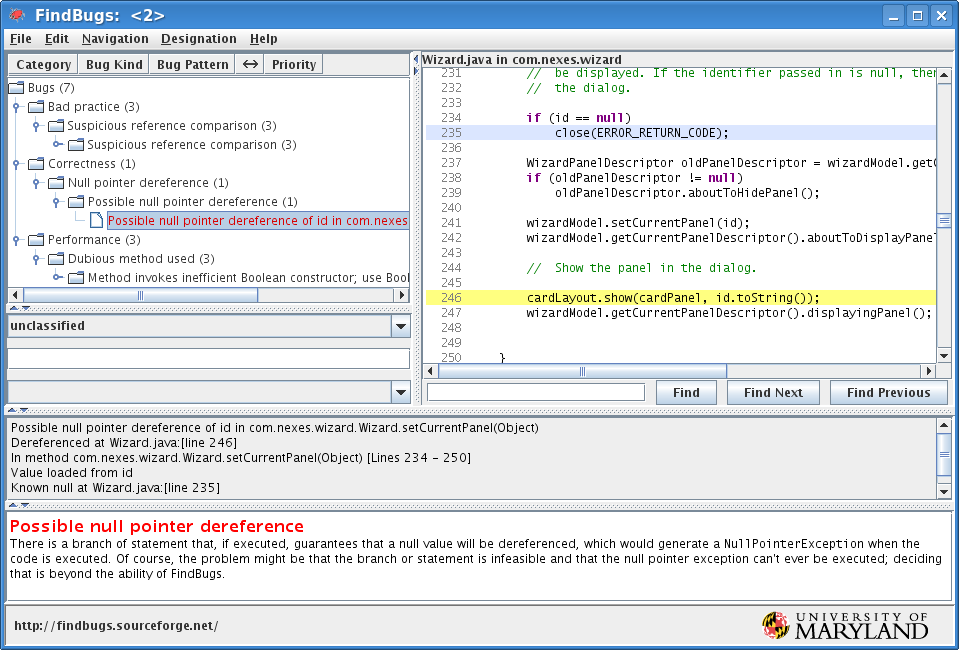
\includegraphics[width=\linewidth]{qm/findbugs}
\else
\begin{figure}[H]
\centering
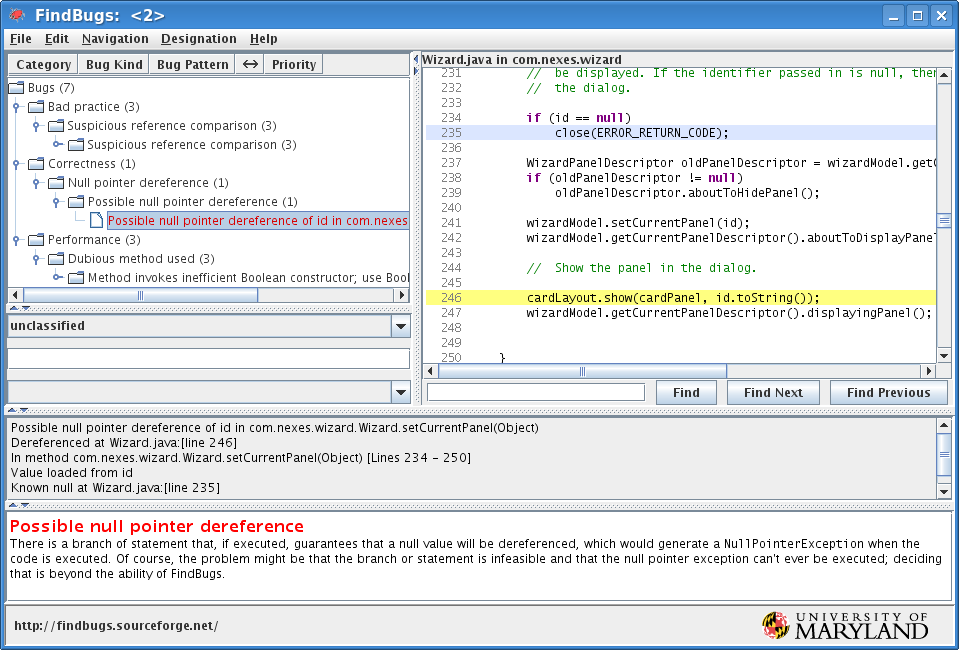
\includegraphics[width=0.9\linewidth]{qm/findbugs}
\caption{FindBugs User Interface}
\end{figure}
\fi
%
\newslide
\subsection{Checkstyle}
Checkstyle is a development tool to help programmers write Java
code that adheres to a coding standard. It automates the process
of checking Java code to spare humans of this boring (but important)
task. This makes it ideal for projects that want to enforce a
coding standard.\\
Checkstyle could be integrated in all major development environments
(e.g. IntelliJ, Eclipse, Netbeans). It is also possible to use
Checkstyle as an independent tool:
 \begin{lstlisting}[language=csh]
% java -jar checkstyle-all-4.4.jar \
     -c checkstyle-4.4/sun_checks.xml
     -r src/
 \end{lstlisting}
 In this example the code located in the \verb|src| directory will be
 checked against the rules defined in the \verb|sun_checks.xml| file.

 \vspace{3mm}

With Ant:
\begin{lstlisting}[language=xml]
  <target name="checkstyle">
    <checkstyle config="checkstyle-4.4/sun_checks.xml">
       <fileset dir="src" includes="**/*.java" />
    </checkstyle>
  </target>
\end{lstlisting}

\vspace{3mm}

With Maven:
\begin{lstlisting}[language=xml,
  morekeywords={reporting,plugins,plugin,groupId,artifactId,configuration}]
  <reporting>
    <plugins>
      <plugin>
        <groupId>org.apache.maven.plugins</groupId>
        <artifactId>maven-checkstyle-plugin</artifactId>
        <configuration>config/sun_checks.xml</configuration>
      </plugin>
    </plugins>
  </reporting>
\end{lstlisting}
\newpage

Example:
\begin{figure}[H]
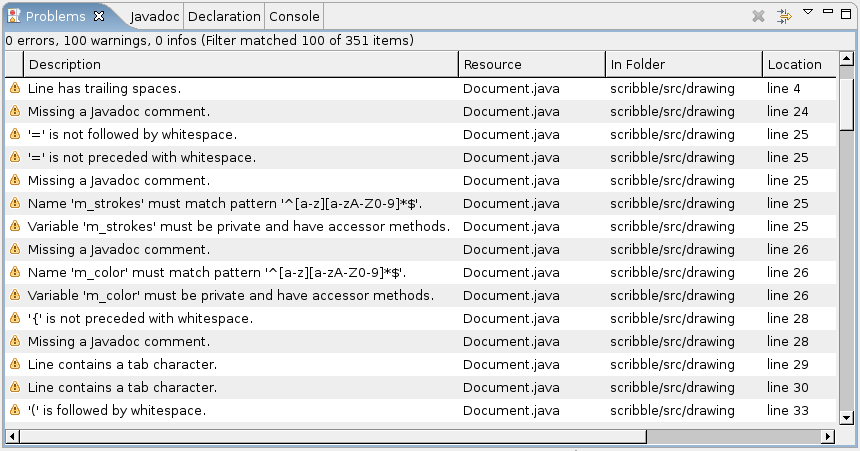
\includegraphics[width=\linewidth]{qm/checkstyle}
\caption{Checkstyle-Eclipse-Plugin}
\end{figure}
%
\newslide
\section{Assertions}
An assertion is a statement in Java which ensures the correctness of
any assumptions which have been done in the program. When an assertion
is executed, it is assumed to be true. If the assertion is false,
the Java Virtual Machine will throw an Assertion error. It finds it application
primarily in the testing purposes. Assertion statements are used
along with boolean expressions.

\begin{lstlisting}[language=java, morekeywords={assert}]
  double d = 4 * a * c - b*b;
  assert d >= 0 : "Negative Value";
  double x1 = sqrt( d );
\end{lstlisting}

By default, assertions are disabled in Java. In order to enable them we use
the vm parameter \verb|ea|:

\begin{lstlisting}[language=csh]
% java -ea AssertionTest
\end{lstlisting}

%
\newslide
\section{Logging und Tracing}
A large part of software developers lives are monitoring,
troubleshooting and debugging.\\
The possibility to reproduce a bug on the local development
machine makes it easier to find the root cause. A debugger
could be used to walk through the code, step by step.\\
If it is not possible to reproduce the bug on the local
development environment makes it very hard.\\
Proper logging makes this a much easier and smoother process.\\
There are several reasons for logging:

\begin{itemize}
\item Error handling
\item Monitoring
\item Auditing
\end{itemize}

Statements like \verb|System.out.println()| should not be used. There
are frameworks available for that. A very popular one is Apache Log4J.

\vspace{3mm}

Example:
\begin{lstlisting}[language=java]
package drawing;
import org.apache.log4j.Logger;

public class Scribble{
  final Logger logger = Logger.getLogger(Scribble.class);
  public Scribble(){
    logger.trace("Entering drawing mode..");
    logger.debug("Start a new drawing");
    logger.info("Connected to database");
    logger.warn("Empty input");
    logger.error("Permission denied");
    logger.fatal("Exhausted memory");
  }
}
\end{lstlisting}



\subsection{Configuration}
The display of the messages, the format and the target (file, console, mail,
database, ...) will be defined in a configuration file. This file
is called \verb|log4j2.xml| and should be placed in the classpath
of the project.

\begin{lstlisting}[language=xml]
<?xml version="1.0" encoding="UTF-8"?>
<Configuration status="DEBUG">
    <Appenders>
        <Console name="LogToConsole" target="SYSTEM_OUT">
            <PatternLayout pattern=
            "%d{HH:mm:ss.SSS} [%t] %-5level %logger{36} - %msg%n"/>
        </Console>
        <File name="LogToFile" fileName="logs/app.log">
            <PatternLayout>
                <Pattern>%d %p %c{1.} [%t] %m%n</Pattern>
            </PatternLayout>
        </File>
    </Appenders>
    <Loggers>
        <Logger name="ch.fhnw" level="debug" additivity="false">
            <AppenderRef ref="LogToFile"/>
            <AppenderRef ref="LogToConsole"/>
        </Logger>
        <Logger name="org.springframework.boot" level="error"
        additivity="false">
            <AppenderRef ref="LogToConsole"/>
        </Logger>
        <Root level="error">
            <AppenderRef ref="LogToFile"/>
            <AppenderRef ref="LogToConsole"/>
        </Root>
    </Loggers>
</Configuration>
\end{lstlisting}

There are many appenders available:

\begin{itemize}
\item ConsoleAppender
\item FileAppender
\item SMTPAppender
\item JDBCAppender
\item JMSAppender
\item NTEventLogAppender
\item TelnetAppender
\item SyslogAppender
\item SocketAppender
\end{itemize}

If a message will appear depends on the defined priority.\\
The following log levels are available:

\begin{tabularx}{\linewidth}{llX}
0 & TRACE & Designates finer-grained informational events than the DEBUG. \\
1 & DEBUG & Designates fine-grained informational events that are most useful to debug an application.\\
2 & INFO & Designates informational messages that highlight the progress of the application at coarse-grained level.\\
3 & WARN & Designates potentially harmful situations.\\
4 & ERROR & Designates error events that might still allow the application to continue running.\\
5 & FATAL & Designates very severe error events that will presumably lead the application to abort.\\
\end{tabularx}

There could be more or less levels available, depending on the
used log framework.
The following format options are available to set up the format
of a message:

%Die folgenden Formatierungsanweisungen können für die Festlegung des
%Ausgabeformates verwendet werden:

\begin{tabularx}{\linewidth}{lX}
\%n & newline\\
\%m & your log message\\
\%p & message priority (FATAL, ERROR, WARN, INFO, DEBUG, TRACE \ldots)\\
\%r & millisecs since program started running\\
\%\% & percent sign in output\\
\%c & name of your category (logger)\\
\%t & name of current thread\\
\%d & date and time\\
\%l & Shortcut for \%F\%L\%C\%M\\
\%F & Java source file name\\
\%L & Java source line number\\
\%C & Java class name\\
\%M & Java method name\\
\end{tabularx}
%
\subsection{Logging versus Debugging}
Brian W. Kernighan, Rob Pike, ``The Practice of Programming'' (1999):
\begin{quote}
As a personal choice, we tend not to use debuggers beyond getting a stack trace
or the value of a variable or two. One reason is that it is easy to get lost
in details of complicated data structures and control flow; we  find stepping
through a program less productive than thinking harder and adding output
statements and self-checking code at critical places. Clicking over statements
takes longer than scanning the output of judiciously-placed displays. It takes
less time to decide where to put print statements than to single-step to the
critical section of code, even assuming we know where that is. More important,
logging statements stay with the program; debugging sessions are
transient.
\end{quote}
%
\newslide
\subsection{Other frameworks}
Together with the Spring Boot technology, the logging framework \emph{Logback}
is avaiable.\\
Logback is intended as a successor to the popular log4j project,
picking up where log4j leaves off.

\vspace{3mm}

There is a default configuration available which could be configured
in different ways:

First, we can set our logging level within our VM Options:

\begin{lstlisting}
-Dlogging.level.org.springframework=INFO
-Dlogging.level.ch.fhnw=TRACE
\end{lstlisting}

or with Maven:

\begin{lstlisting}
mvn spring-boot:run
  -Dspring-boot.run.arguments=
    --logging.level.org.springframework=INFO,
    --logging.level.ch.fhnw=TRACE
\end{lstlisting}

If there is a configuration file \verb|logback.xml| in the classpath,
the default configuration will be overwritten by that file:

\begin{lstlisting}[language=xml]
<?xml version="1.0" encoding="UTF-8"?>
<configuration>

    <property name="LOGS" value="./logs" />

    <appender name="Console"
        class="ch.qos.logback.core.ConsoleAppender">
        <layout class="ch.qos.logback.classic.PatternLayout">
            <Pattern>
                %black(%d{ISO8601}) %highlight(%-5level)
                [%blue(%t)] %yellow(%C{1.}): %msg%n%throwable
            </Pattern>
        </layout>
    </appender>

    <appender name="RollingFile"
        class="ch.qos.logback.core.rolling.RollingFileAppender">
        <file>${LOGS}/spring-boot-logger.log</file>
        <encoder
            class="ch.qos.logback.classic.encoder.PatternLayoutEncoder">
            <Pattern>%d %p %C{1.} [%t] %m%n</Pattern>
        </encoder>

        <rollingPolicy
            class="ch.qos.logback.core.rolling.TimeBasedRollingPolicy">
            <!-- rollover daily and when the file reaches 10 MegaBytes -->
            <fileNamePattern>
            ${LOGS}/archived/spring-boot-logger-%d{yyyy-MM-dd}.%i.log
            </fileNamePattern>
            <timeBasedFileNamingAndTriggeringPolicy
                class="ch.qos.logback.core.rolling.SizeAndTimeBasedFNATP">
                <maxFileSize>10MB</maxFileSize>
            </timeBasedFileNamingAndTriggeringPolicy>
        </rollingPolicy>
    </appender>

    <!-- LOG everything at INFO level -->
    <root level="info">
        <appender-ref ref="RollingFile" />
        <appender-ref ref="Console" />
    </root>

    <logger name="ch.fhnw" level="trace" additivity="false">
        <appender-ref ref="RollingFile" />
        <appender-ref ref="Console" />
    </logger>

</configuration>
\end{lstlisting}

%
\newslide
\section{Vergleiche von Textdateien}
Vergleiche von Textdateien sind oft nicht einfach, wenn man dazu
nicht einen spezialisierten Texteditor (z.B Emacs, what else?) verwenden will.
Unter den Unix-Werkzeugen gibt es jedoch zwei Programme, die
uns diese Aufgabe vereinfachen: diff und cmp.

\newslide
Beispiel:
\begin{lstlisting}[basicstyle=\small]
$ diff colors1.txt colors2.txt

 6c6
 < # indigo
  ---
  > # indigo-blue
  11d10
  < # sienna
  12a12
  > # darkblue
  15c15
  < # tomato
  ---
  > # tomato-red
\end{lstlisting}
\newslide
Die Ausgabe erscheint auf den ersten Blick etwas verwirrend.
Versuchen wir es nochmals mit der Option -u (unified):
\begin{lstlisting}
$ diff -u colors1.txt colors2.txt

  --- colors1.txt 2005-04-01 20:45:21.954828407 +0200
  +++ colors2.txt 2005-04-01 20:44:50.152742422 +0200
  @@ -3,13 +3,13 @@
  # darkred
  # deeppink
  # firebrick
  -# indigo
  +# indigo-blue
  # limegreen
  # royalblue
  # sandybrown
  # seagreen
  -# sienna
  # silver
  +# darkblue
  # skyblue
  # teal
  -# tomato
  +# tomato-red
\end{lstlisting}
Die Unterschiede sind nun offensichtlicher. Die abweichenden
Zeilen sind mit den Zeichen \verb+-+ und \verb|+| markiert.
In der ersten Datei steht ''indigo''
in der zweiten ''indigo-blue''. Der zweiten Datei fehlt der Eintrag
sienna, dafür gibt es darkblue, etc. etc.

\newslide
Eine noch bessere Übersicht hat man mit
\begin{lstlisting}
$ diff -y -W 50 colors1.txt colors2.txt

# chocolate             # chocolate
# crimson               # crimson
# darkred               # darkred
# deeppink              # deeppink
# firebrick             # firebrick
# indigo              | # indigo-blue
# limegreen             # limegreen
# royalblue             # royalblue
# sandybrown            # sandybrown
# seagreen              # seagreen
# sienna              <
# silver                # silver
                      > # darkblue
# skyblue               # skyblue
# teal                  # teal
# tomato              | # tomato-red
\end{lstlisting}
Das Zeichen \verb+|+ zeigt eine Abweichung an und die Zeichen
\verb+>+ und  \verb+<+ teilen mit, dass in der ersten
respektive zweiten Datei ein zusätzlicher
Eintrag vorhanden ist.
Die Option -y
steht für ''nebeneinander'' während die Option ''-W 50''
die Spaltenbreite setzt.

\newslide
Damit scheint diff für Textvergleiche am besten geeignet zu sein.
Mit dem Programm cmp kann keine annähernd so übersichtliche
Ausgabe erzeugt werden:
\begin{lstlisting}
$ cmp colors1.txt colors2.txt

 colors1.txt colors2.txt differ: byte 64, line 6
\end{lstlisting}
Wenn es jedoch lediglich darum geht herauszufinden, ob
Abweichungen vorhanden sind, kann dies vorteilhafter sein.

Quelle:
\href{http://www.brunolinux.com/02-The_Terminal/Diff_and_Cmp.html}
{www.brunolinux.com/02-The\_Terminal/Diff\_and\_Cmp.html}
\newslide
\section{Integritätsprüfung mit Md5sum}
Die MD5-Summen (RFC 1321)
aller in im aktuellen Verzeichnis und darunter
liegenden Dateien können auf einem Unix-System mit folgender Anweisung
in eine Textdatei geschrieben werden:
\begin{lstlisting}
$ find . -type f 2>/dev/null -exec md5sum {} \; >test.md5
\end{lstlisting}
Diese Datei könnte beispielsweise folgende Zeilen enthalten:
\begin{lstlisting}
f3dd21a2023813be41c9f4b879783d38  ./colors.txt
9dab480789443d080d347138acdad7e5  ./quick_ref.pdf
f91449e7f5661b64c568a6c8a8834224  ./Console-Colors
a1ef1c1dc94d5a6d44dd5e0678f436a8  ./dsp.sxw
..
\end{lstlisting}
%$
\newslide
Es handelt sich um 128-Bit-Hashwerte, die man auch als
''Fingerabdruck'' einer Datei bezeichnet.
Die so erstellte Datei test.md5 kann nun verwendet werden,
um zu einem späteren Zeitpunkt
zu prüfen, ob sich etwas geändert hat (Integritätsprüfung):
\begin{lstlisting}
  md5sum -c test.md5
\end{lstlisting}
Quelle: \href{http://www.brunolinux.com/02-The_Terminal/Diff_Find_and_Md5sum.html}
  {www.brunolinux.com/02-The\_Terminal/Diff\_Find\_and\_Md5sum.html}
%
\newslide
\section{Unit-Test}
\subsection{JUnit}
JUnit ist ein einfaches und mächtiges Java-Framework für die
Entwicklung und das Ausführen von Unit-Tests.
%Mit Hilfe von Klassenbibliotheken wie
%CppUnit \href{http://CppUnit.sourceforge.net}{CppUnit.sourceforge.net} oder
%JUnit \href{http://JUnit.org}{JUnit.org}
%lassen sich Unit-Tests weitgehend automatisieren.

Man geht dazu wie folgt vor:
\begin{enumerate}
\item Man erstellt eine Klasse K
  (z.B. SimpleTest), die von TestCase abgeleitet
 ist:
\begin{lstlisting}[language=java]
import java.util.*;
import junit.framework.*;

public class SimpleTest extends TestCase {

}
\end{lstlisting}
\newslide
\item Für jeden Test XXX wird eine Methode \lstinline{void testXXX()}
  definiert,
  in welcher Soll- und Ist-Werte mittels \lstinline{assertEquals( soll, ist )}
   verglichen werden
  oder allgemein mit

\lstinline{assertTrue( bool exp )}

auf die Bedingung \verb+true+ getestet wird.
\begin{lstlisting}[language=java]
  public void testEmptyCollection() {
    Collection collection = new ArrayList();
    assertTrue(collection.isEmpty());
  }
 \end{lstlisting}
  Beim Testen von Gleitkommawerten kann mit der Methode
  \lstinline{assertEquals( soll, ist, delta )} geprüft werden, ob die Werte
  innerhalb des mit delta festgelegten Intervalles liegen.
\newslide
\item Die Methoden \verb|setUp()| und \verb|tearDown()|
können für die Instantiierung und das Aufräumen
  der Testobjekte verwendet werden. Dies wird auch Fixture (engl.
  Vorrichtung) genannt.
\item Mit der Methode \verb+suite()+ wird eine TestSuite erstellt,
  die dank dem Java-Reflection-Mechanismus automatisch alle test-Methoden
  aufruft:
\begin{lstlisting}[language=java]
  public static Test suite() {
    return new TestSuite(SimpleTest.class);
  }
\end{lstlisting}
\newslide
\item Schlussendlich wird noch die main-Funktion benötigt:
\begin{lstlisting}[language=java]
  public static void main(String args[]) {
    junit.textui.TestRunner.run(suite());
  }
\end{lstlisting}
\end{enumerate}
Mit der Anweisung:
\begin{verbatim}
% java junit.swingui.TestRunner SimpleTest
\end{verbatim}
wird ein grafisches Frontend gestartet,
die TestSuite ausgeführt und die Ergebnisse angezeigt.
\begin{figure}[H]
\begin{center}
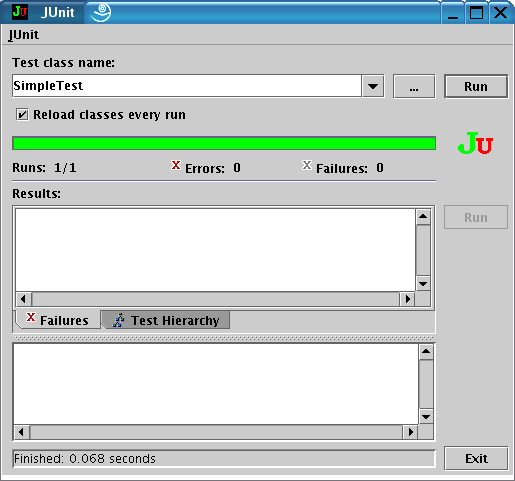
\includegraphics[width=0.6\linewidth]{qm/guitestrunner}
\end{center}
\caption{JUnit TestRunner}
\end{figure}
\ifslides
\newpage
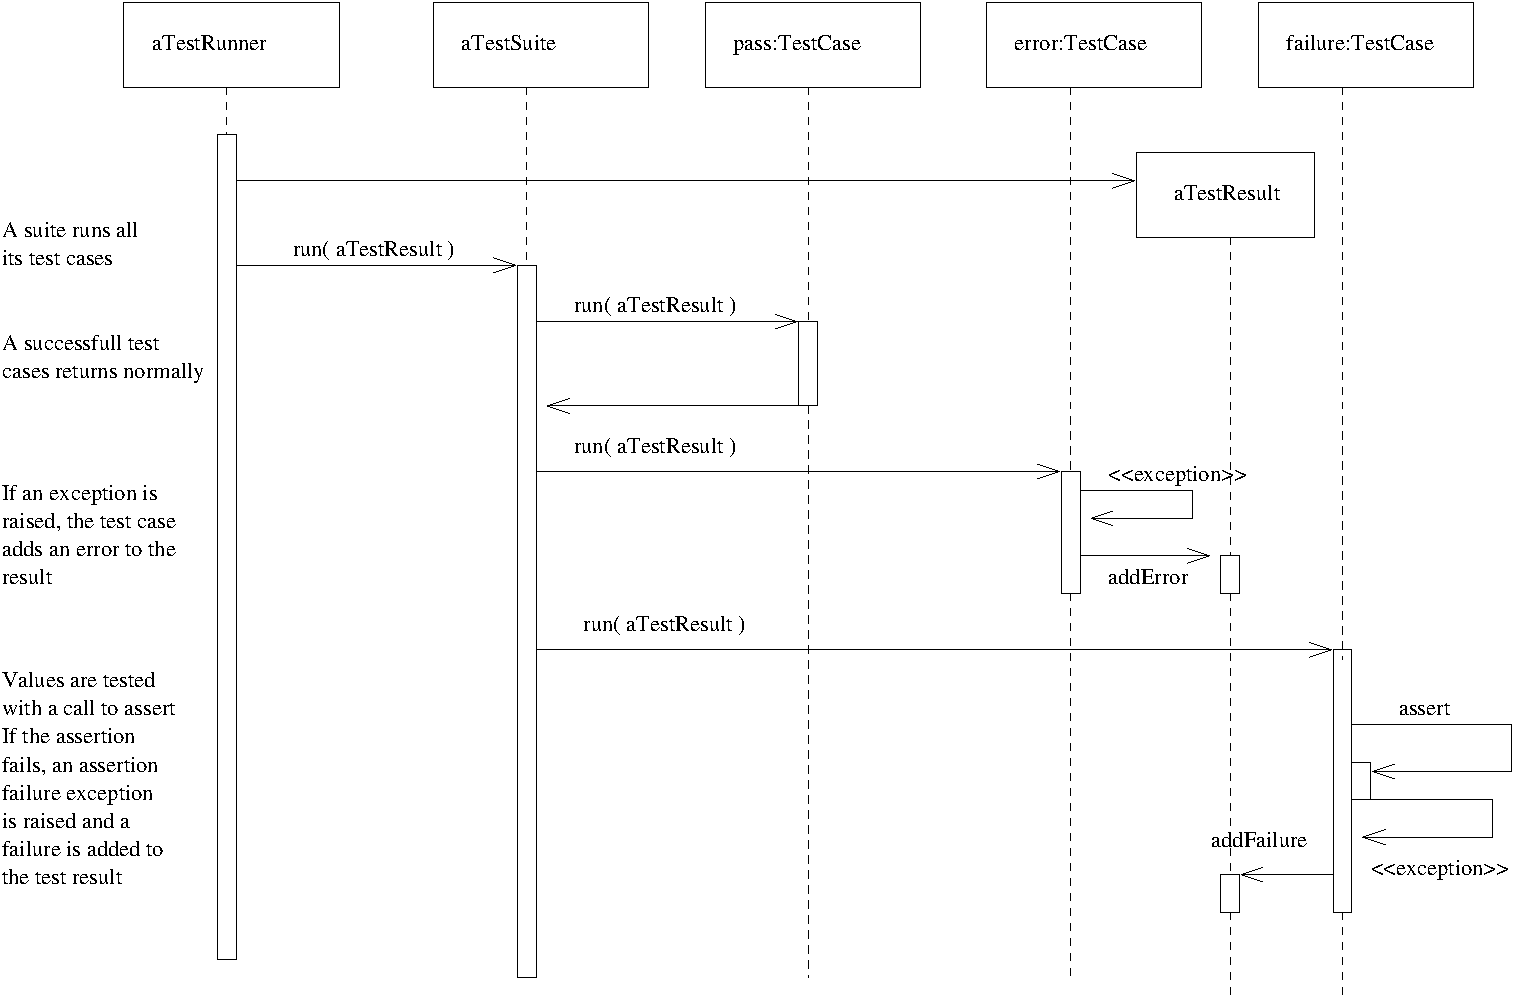
\includegraphics[width=\linewidth]{qm/xfig/cppunit-seq}
\else
\begin{figure}[H]
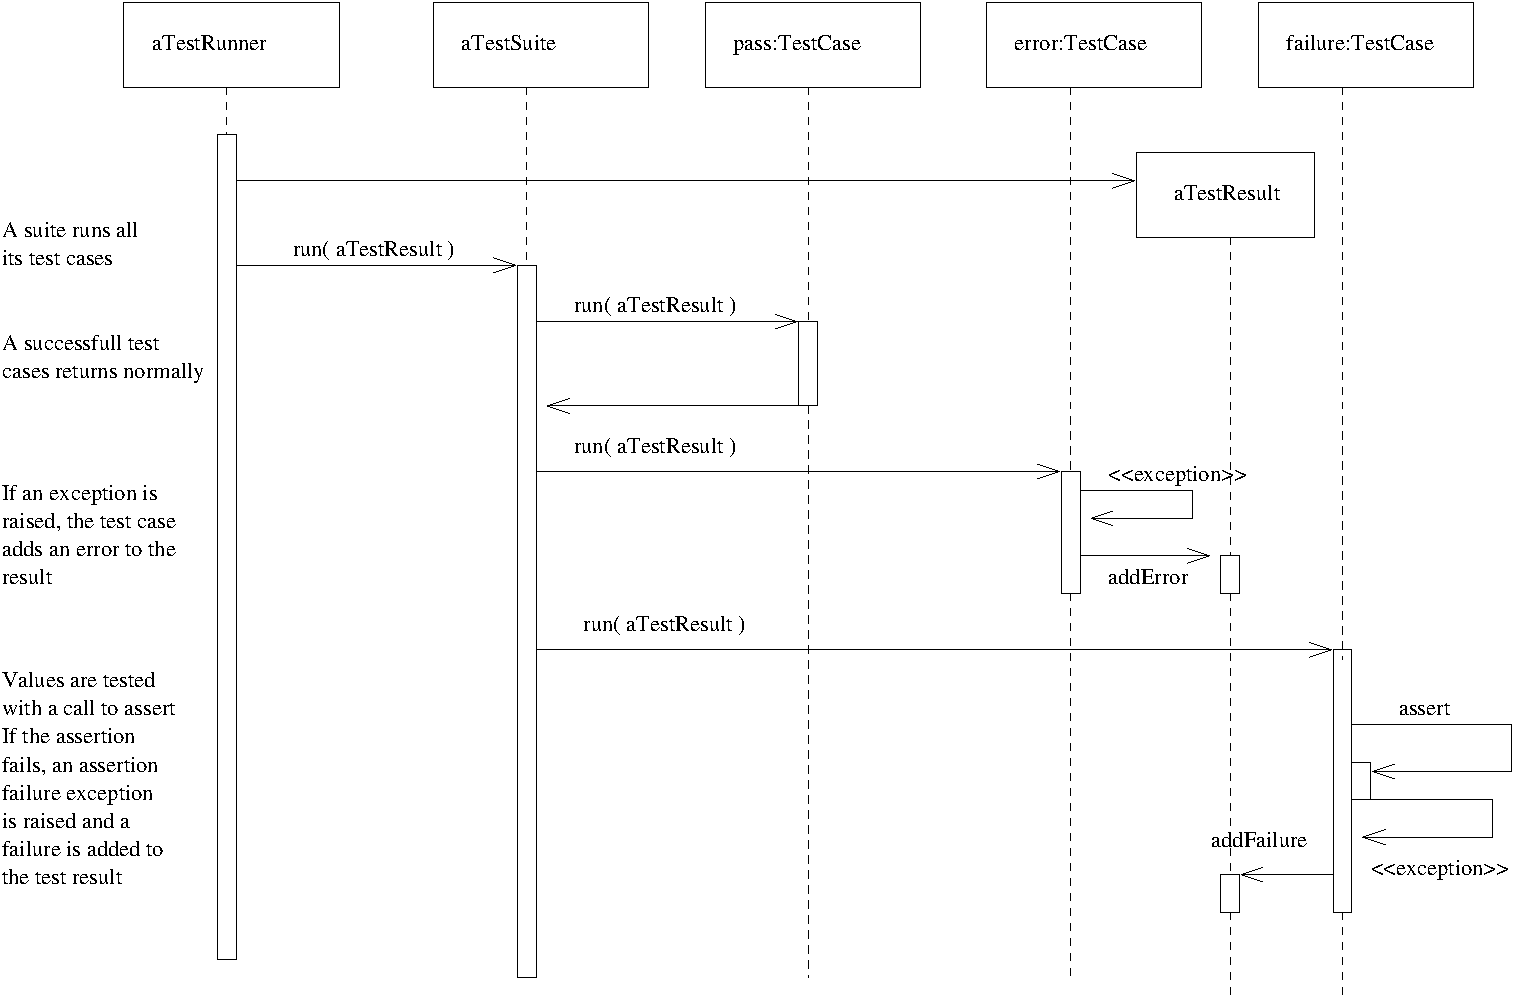
\includegraphics[width=\linewidth]{qm/xfig/cppunit-seq}
\caption{JUnit Sequenzdiagramm}
\end{figure}
\fi

Noch einfacher geht es mit Eclipse:
\begin{enumerate}
\item File $\longrightarrow$ New $\longrightarrow$ Junit Test Case

 Es erscheint das Dialog-Fenster ``New JUnit Test Case''. Hiermit
lässt sich die TestCase-Klasse erzeugen. Es empfiehlt sich jedoch
die Warnung

``JUnit .. is not on the build path...''

zu beachten und mit ``Click here'' die Archiv-Datei dem Build-Pfad
hinzu zufügen.
\newslide
\item Man schreibt eine Test-Methode. Z.B:
\begin{lstlisting}[language=java]
  public void testEmptyCollection() {
    Collection collection = new ArrayList();
    assertTrue(collection.isEmpty());
  }
 \end{lstlisting}
\newslide
\item Man kreiert einen neuen JUnit-Test:

Run $\longrightarrow$ Run\ldots $\longrightarrow$ JUnit $\longrightarrow$ New

\item Man führt den Test aus.
\end{enumerate}
\newslide
Es empfiehlt sich grundsätzlich mit der Entwicklung von Tests zu beginnen und
 erst anschliessend die entsprechende Klasse zu implementieren.
Dies wird als test-getriebenes Vorgehen bezeichnet:
abwechslungsweise
ein wenig kodieren und dann wieder ein wenig testen. Oder
wie es Bill Wake \footnote{Extreme Programming Explored}
sehr zutreffend ausdrückt:
\begin{quote}
There's a rhythm to it, like a pendulum of a clock: test a little,
code a little, test a little, code a little.
\end{quote}
Die Klassen
 werden dadurch einfacher testbar und zudem verbessert sich auch ganz generell
 das Programmdesign. Diese Methode wird auch Test-Driven-Development (TDD)
 genannt.
\newslide
Wem das alles bereits zu fundamentalistisch vorkommt,
der kann sich ja an das
\href{http://www.developertesting.com/archives/month200702/20070206-000391.html}
{Testivus-Manifest}
von Alberto Savoia halten:
\begin{itemize}
\item Less testing dogma, more testing karma.
\item Any tests are better than no tests.
\item Testing beats debugging.
\item Test first, during, or after -- whatever works best for you.
\item If a method, technique, or tool, gives you more or better tests use it.
\end{itemize}
%
\newslide
\subsection{Junit4}
Die aktuelle Verion 4 von Junit bietet gegenüber der Version 3.8
die folgenden Verbesserungen:
\begin{itemize}
\item POJO-Klassen mit Annotationen statt Ableiten von TestCase:
\begin{itemize}
\item \textcolor{red}{@Test} kennzeichnet Methoden als ausführbare Testfälle.
\item \textcolor{red}{@Before} und \textcolor{red}{@After}
  markieren Setup- bzw. Teardown-Aufgaben, die
  für jeden Testfall wiederholt werden sollen.
\item \textcolor{red}{@BeforeClass} und \textcolor{red}{@AfterClass}
  markieren Setup-
  bzw. Teardown-Aufgaben, die nur einmal pro Testklasse ausgeführt
  werden sollen.
\end{itemize}
\item Testen von Exceptions und Timeouts
\end{itemize}
\newslide
\begin{lstlisting}[language=java,escapechar=\%]
import org.junit.Assert;
import org.junit.After;
import org.junit.Before;
import org.junit.Test;

public class SimpleTest {

    %\textcolor{red}{@Before}%
    public void setUp() throws Exception {
    }

    %\textcolor{red}{@After}%
    public void tearDown() throws Exception {
    }

    %\textcolor{red}{@Test}%(expected=ArrayIndexOutOfBoundsException.class)
    public void indexOutOfRange(){
      double x[] = new double [1];
      x[1]=0;
    }

    %\textcolor{red}{@Test}%
    public void testDummy(){
      Assert.assertEquals(1,2);
    }
}
\end{lstlisting}
%Durch die Anweisung \lstinline[language=java]{import static
%    Assert.assertEquals} kann vereinfacht geschrieben werden
%  assertEquals(1,2)
%
%Ein Nachteil von Junit4 ist die noch fehlende Unterstützung in Ant.
%
\newslide
\subsection{TestNG}
In eine ähnliche Richtung wie Junit4 geht auch TestNG. TestNG
 bietet jedoch noch einige zusätzliche Möglichkeiten:
\begin{itemize}
\item XML-Konfiguration
\item Gruppierung von Tests
\item Festlegung von Abhängigkeiten, paralleles Testen
\item parametrisiertes Testen
\end{itemize}
\newslide
Beispiel:
\begin{lstlisting}[language=java,escapechar=\%]
import org.testng.annotations.AfterTest;
import org.testng.annotations.BeforeTest;
import org.testng.annotations.Test;


public class SimpleTest {

  %\textcolor{red}{@BeforeTest}%
  public void setUp() throws Exception {
  }

  %\textcolor{red}{@AfterTest}%
  public void tearDown() throws Exception {
  }

  %\textcolor{red}{@Test}%(expectedExceptions=ArrayIndexOutOfBoundsException.class)
  public void indexOutOfRange(){
    double x[] = new double [1];
    x[1]=0;
  }

  %\textcolor{red}{@Test}%
  public void testDummy(){
    assert 1==2;
  }
}
\end{lstlisting}
\newslide
\subsection{Mock-Objekte}
Beim Unit-Testen ist man darauf angewiesen, dass die Methoden der zu testenden
Klasse weitgehend von der Umgebung isoliert ausgeführt werden
können. Leider kann diese Voraussetzung in den meisten Fällen nicht
erfüllt werden. Oft sind die
Klassen auf vielfältige Art mit weiteren Klassen oder Systemen wie zum
Beispiel Filesystemen, Datenbanken, Web-Server, Netzwerken,
Hardware-Schnittstellen etc. verbunden. Will man solche Klassen
testen, bedeutet es, dass man sie von der ``realen'' Umgebung
abschirmt. Am einfachsten
macht man dies mit Hilfe von Attrappen, die in die
Testobjekte eingeschleust werden. Wenn man das richtig macht, können
Attrappen dafür sorgen, dass die
Tests in einer deterministischen Umgebung ablaufen.

\newslide
Ein einfache Attrappe, ``Dummy'' oder ``Stub'' genannt, müsste keine
eigene Logik enthalten, sondern einfach zweckmässige Resultate zurück geben
zum Beispiel in Form  konstanter Werte.

Eine interessantere Variante solcher
Attrappen sind jedoch Mock-Objekte. Darunter versteht man Objekte, die ein
Endo-Testen ermöglichen, also ein Testen von Innen.

\newslide
Dies soll anhand von folgendem, vereinfachten Beispiel erläutert werden:
\begin{lstlisting}[language=java]
public class RFIDReader {
  private SerialPort port;
  private boolean errorFlag;

  public RFIDReader(){
    errorFlag=false;
    port = new SerialPort("COM1", 9600 );
    port.open();
  }
\end{lstlisting}
\newslide
Die Methode list gibt die gelesenen Tags auf der Konsole aus:
\begin{lstlisting}[language=java]
  public void list(){
    String rfidTag;
    try{
      while ((rfidTag = port.read()) != null) {
        System.out.println( rfidTag );
      }
    }
    catch( ReadError ex ){ errorFlag=true;}
    port.close();
  }
\end{lstlisting}
\newslide
Mit isError kann auf Lesefehler geprüft werden:
\begin{lstlisting}[language=java]
public boolean isError(){
    return errorFlag;
  }
}
\end{lstlisting}
\newslide
Mit der Klasse RFIDReader können RFID-Tags (Radio Frequency Identifier), die
von einer seriellen Schnittstelle gelesen werden, auf der Konsole ausgegeben
werden:
\begin{lstlisting}[language=java]
  RFIDReader reader = new RFIDReader();
  reader.list();
\end{lstlisting}
\newslide
Diese Klasse lässt sich eigentlich kaum mit JUnit testen:
\begin{itemize}
\item Das SerialPort-Objekt ist fest vorgegeben im Konstruktor.
\item Die Rückgabewerte der read-Methode sind nicht beeinflussbar und damit
  nicht deterministisch.
\item Die Ausgabe wird auf System.out geschrieben.
\end{itemize}
\newslide
Mit den folgenden Modifikationen kann die Klasse mit JUnit getestet werden:
\begin{itemize}
\item Das Port-Objekt wird durch ein Interface beschrieben und dem Konstruktor
  oder einer setter-Methode als Argument übergeben:
\newslide
  \begin{lstlisting}[language=java]
public interface Port {
  public void open();
  public String read() throws ReadError;
  public void close();
}

public class RFIDReader {
  private Port port;
  public RFIDReader(Port p){
    errorFlag=false;
    port = p;
  }
  ..
  \end{lstlisting}
\newslide
\item Die List-Methode verwendet ein Stream-Objekt für die Ausgabe:
  \begin{lstlisting}[language=java]
    ..
  public void list( PrintStream out ){
    String rfidTag;
    try{
      while ((rfidTag = port.read()) != null) {
        out.println( rfidTag );
      }
    }
    catch( ReadError ex ){
      errorFlag=true;
    }
    port.close();
  }
  ..
  \end{lstlisting}
\end{itemize}
Dadurch liesse sich beispielsweise der folgende Test ausführen:
\begin{lstlisting}[language=java]
  ...
    public void testReader(){
        MockPort mockport = new MockPort();
        RFIDReader r = new RFIDReader( mockport );
        r.list( mockport );
        mockport.verify();
    }
  ...
\end{lstlisting}
Die eigentlichen Tests erfolgen nun im Mock-Objekt selbst.

\newslide
Damit die Ausgabe der List-Methode geprüft werden kann, muss
die Klasse von PrintStream abgeleitet sein und das Interface Port
implementieren:
\begin{lstlisting}[language=java]
..
import junit.framework.Assert;

public class MockPort extends PrintStream implements Port{
    private ArrayList list;
    private Iterator outIterator;
    private Iterator inIterator;
    private boolean isClosed;
    private boolean isOpen;

..
}
\end{lstlisting}
\newslide
Im Konstruktor wird eine Liste mit RFID-Tags erstellt, die
beim Read-Aufruf zurückgegeben werden:
\begin{lstlisting}[language=java]
public MockPort() {
        super(System.out);
        list = new ArrayList();
        list.add("E004010002035FE7");
        list.add("0900000033E52E12");
        list.add("E004010002035BFB");
        inIterator = list.iterator();
        outIterator = list.iterator();
    }
\end{lstlisting}
\newslide
Die Read-Methode gibt bei jedem Aufruf das nächste Element der
Tag-Liste
zurück:
\begin{lstlisting}[language=java]
  public String read() throws ReadError {
        if( !inIterator.hasNext() ){
            return null;
        }
        return (String)inIterator.next();
    }
  \end{lstlisting}
\newslide
Die Print-Methode überprüft nun, ob die RFID-Tags in der richtigen
Reihenfolge eintreffen:
\begin{lstlisting}[language=java]
  public void println( String s ){
        if( !outIterator.hasNext() ){
            Assert.fail("overrun");
        }
        if( !s.equals( (String)outIterator.next())){
            Assert.fail("changed sequence");
        }
    }
  \end{lstlisting}
\newslide
Weitere Tests wären mit den Funktionen open und close möglich:
\begin{lstlisting}[language=java]
  public void open() {
        isOpen=true;
        isClosed=false;
    }

    public void close() {
        isClosed=true;
        isOpen=false;
    }
  \end{lstlisting}
\newslide
Nach Beendigung der Tests kann verify zum Beispiel prüfen, ob
der Port geschlossen wurde:
\begin{lstlisting}[language=java]
public void verify(){
        if( !isClosed ){
            Assert.fail( "port not closed");
        }
    }
}
\end{lstlisting}
{\bfseries Fazit:} Mit Hilfe von Mock-Objekten lassen sich auch komplexe
Klassen bis ``in den hintersten Winkel'' austesten.
Der einzige Nachteil beim Testen mit Mock-Objekten ist der Aufwand,
der nötig wird, um diese Klassen zu implementieren. Hier können
jedoch Frameworks Abhilfe schaffen.
\newslide
Zum Beispiel EasyMock:
Mock-Objekte lassen sich auf der Basis von Interfaces zur Laufzeit
erzeugen:
\begin{lstlisting}[language=java]
import org.easymock.EasyMock;

public class RFIDReaderTest {
  private Port mock;
  private RFIDReader reader;

  @Before
  public void setUp() {
    mock = EasyMock.createMock(Port.class);
    reader = new RFIDReader(mock);
  }
\end{lstlisting}
\newslide
Wenn man einen Testfall schreibt, muss man zunächst dem Mock-Objekt mitteilen,
welche Methoden in welcher Reihenfolge aufgerufen werden
und welche Ergebnisse sie zurückliefern sollen:
\begin{lstlisting}[language=java]
  @Test
  public void testReader() throws ReadError{
    String expectedTags[] ={
      "E004010002035FE7",
      "0900000033E52E12",
      "E004010002035BFB"
    };
    for( int i=0; i<expectedTags.length; i++){
      EasyMock.expect(mock.read()).andReturn( expectedTags[i] );
    }
    EasyMock.expect( mock.read() ).andReturn( null );
    mock.close();
    EasyMock.replay( mock );

    String returnedTags[] = reader.getTags();
    Assert.assertEquals( "number of RFID tags",
                  expectedTags.length, returnedTags.length);
    EasyMock.verify( mock );
 }
\end{lstlisting}
Nachdem man die Methode replay() aufgerufen hat, kann der Test
durchgeführt werden.

\newslide
Zur Vereinfachung wurde hier die Methode getTags()
der RFIDReader-Klasse hinzugefügt:
\begin{lstlisting}[language=java]
  public String [] getTags() {
    ArrayList<String> list = new ArrayList<String>();

    try{
      String rfidTag;
      while ((rfidTag=port.read() ) != null) {
        list.add( rfidTag );
      }
    }
    catch( ReadError ex ){
      errorFlag=true;
    }
    String receivedTags[] = new String[ list.size()];
    list.toArray( receivedTags );
    return receivedTags;
  }
\end{lstlisting}
Sie gibt einen String-Array mit den gelesenen RFID-Tags zurück.
%-------------------------------------------------------------------------
\newslide
\subsection{DBUnit}
Die grundsätzliche Problematik beim Testen von Datenbank-Code
beschreibt Richard Dallaway sehr anschaulich:
\href{http://www.dallaway.com/acad/dbunit.html}
{www.dallaway.com/acad/dbunit.html}
\begin{quote}
I'm guessing some, if not a lot, of database development goes like
this: set up database, write code to access database, run code, do a
SELECT to see if the records showed up in the database. They did?
Good, then we're done.
\end{quote}
Die visuelle Überprüfung von Testergebnissen ist mühsam und wird oft
nicht mit der nötigen Sorgfalt gemacht. Wenn nach einigen Wochen oder
Monaten derselbe Test wieder durchgeführt wird, hat man meist
vergessen, worauf speziell zu achten ist\ldots

\newslide
Auch hier ist der
Einsatz eines automatisierbaren Testsystemes
angebracht.

\begin{quote}
Automated tests — painless tests that run often and test lots — reduce
the chances of your data is going missing. I find they make it easier
for me to sleep at night. (Tests have other positive features: they're
good examples of how to use code, they act as documentation, they make
other people's code less scary when you need to change it, they reduce
debugging time).
\end{quote}

Automatisierte Tests schaffen die Voraussetzung, dass Code
änderbar bleibt.

\newslide
Ein guter Test stellt möglichst geringe Anforderung an seine Umgebung,
er beschafft sich selbst die nötigen Daten und räumt hinterher wieder
auf, so dass keine unerwarteten Seiteneffekte auftreten. Bei
Datenbanken bedeutet dies, dass vor jeder Testdurchführung die Tabellen mit
bestimmten Werten gefüllt werden müssen. Was wiederum zur Folge hat,
dass man in einer typischen Entwicklungsorganisation verschiedene
Datenbanken benötigt:

\newslide
\begin{enumerate}
\item die Produktions-DB: enthält die produktiv verwendeten Daten,
  hier dürfen keine Tests durchgeführt werden,
\item die lokale Entwicklungs-DB: wird zur SW-Entwicklung verwendet,
  in der Regel hat jeder Entwickler seine eigene Version, hier werden
  die meisten Tests ausgeführt, sie enthält nur eine minimale Anzahl von
  Datensätzen,
\item eine Test-DB: wird von mehreren Entwicklern gemeinsam für Tests
  genutzt, enthält eine Kopie der produktiv genutzten Daten,
\item die Integrations-DB: dient der Durchführung der Integrations- und
  System-Tests vor der Inbetriebnahme,
  enthält eine Kopie der produktiv genutzten Daten,
 \end{enumerate}
Dabei muss darauf geachtet werden, dass die
Synchronisation der Datenbankstruktur gewährleistet
ist: d.h., dass allfällige Änderungen der Tabellen, Trigger,
Stored-Procedures, Constraints etc.  in allen Datenbanken
stets korrekt nachgeführt werden.

\newslide
Beispiel:
\begin{lstlisting}[language=java]
public class TestDbAccess {
  private Connection jdbcConnection;
  private IDatabaseConnection conn;

  public TestDbAccess( String name ){
    super(name);
     Class driverClass =
     Class.forName("com.mysql.jdbc.Driver");

   Connection jdbcConnection =
	 DriverManager.getConnection(
	  "jdbc:mysql://localhost/Mondial", "biggus", "dickus");
  }

  @Before
  public void setUp() throws Exception {
    IDataSet dataSet = new FlatXmlDataSet(
                 new FileInputStream("mondial-partial.xml"));
    conn = new DatabaseConnection(jdbcConnection);
    DatabaseOperation.CLEAN_INSERT.execute(conn, dataSet);
  }

  @After
  protected void tearDown() throws Exception {
    conn.close();
  }
 ..
}
\end{lstlisting}
Die Set-Up-Methode sorgt für ein Löschen und Neuladen
der Tabellen vor jedem Test. Dabei wird mit ''mondial-partial.xml''
eine XML-Datei verwendet, die
mit dem DB-Schema der Test-DB korrespondiert:
\begin{lstlisting}[language=xml,morekeywords={dataset}]
<dataset>
  <country Name="Austria" Code="A"
           Capital="Vienna"
           Province="Vienna"
           Area="83850" Population="8023244"/>
  <country Name="Switzerland" Code="CH"
           Capital="Bern" Province="BE"
           Area="41290" Population="7207060"/>
...
</dataset>
\end{lstlisting}
\newslide
\begin{lstlisting}
+------------+-------------+------+-----+---------+
| Field      | Type        | Null | Key | Default |
+------------+-------------+------+-----+---------+
| Name       | varchar(32) | NO   | UNI |         |
| Code       | varchar(4)  | NO   | PRI |         |
| Capital    | varchar(35) | YES  |     | NULL    |
| Province   | varchar(32) | YES  |     | NULL    |
| Area       | int(11)     | YES  |     | NULL    |
| Population | int(11)     | YES  |     | NULL    |
+------------+-------------+------+-----+---------+
\end{lstlisting}
Eine solche Datei kann mit Hilfe von DBUnit aus einer bestehenden
Datenbank generiert werden.

\newslide
Nicht nur einzelne Werte sondern
auch ganze Tabellen können mit DBunit einfach geprüft werden:
\begin{lstlisting}[language=java]
   @Test
   public void testMe() throws Exception {
     // Execute the tested code that modify the database here
     ...
     // Fetch database data after executing your code
     IDataSet databaseDataSet = conn.createDataSet();
     ITable actualTable = databaseDataSet.getTable("Country");
     // Load expected data from an XML dataset
     IDataSet expectedDataSet = new FlatXmlDataSetBuilder().
              build(new File("expectedDataSet.xml"));
     ITable expectedTable = expectedDataSet.getTable("Country");
     // Assert actual database table match expected table
     Assertion.assertEquals(expectedTable, actualTable);
    }
\end{lstlisting}
%\newslide
%\subsection{XML Unit-Test}
%Da XML-Dokumente ganz offensichtlich nicht wie
%andere Textdateien durch einen zeilenweisen Vergleich
%geprüft werden können ..
%
% http://www.infoq.com/articles/xml-unit-test
% http://www.ibm.com/developerworks/java/library/j-cq121906.html
%
%\newpage
\subsection{Testbericht-Generierung mit Ant und Maven}
Sowohl Ant wie auch Maven eignen sich für die automatisierte
Testdurchführung und Generierung der Testreports.

Junit-Tests können mit dem Ant-Task \verb+junit+ durchgeführt werden:
\begin{lstlisting}[language=xml,
  morekeywords={target,path,pathelement,junit,classpath,batchtest,fileset}]
<path id="project.classpath">
  <pathelement path="lib/junit.jar"/>
  <pathelement path="${build.dir}"/>
</path>

<target name="test" depends="compile">
  <junit>
    <classpath refid="project.classpath"/>
    <batchtest>
      <fileset dir="${build.dir}"
               includes="**/*Test.class"/>
    </batchtest>
  </junit>
</target>
\end{lstlisting}
%$
Das Target ''test'' sorgt hier dafür, dass die Testmethoden aller Klassen,
deren Bezeichner mit den Zeichen ``Test'' endet, ausgeführt werden.
\ifslides
\else
(ACHTUNG: Vorgängig muss die Datei junit.jar ins lib-Verzeichnis von Ant
kopiert werden, andernfalls beklagt sich ant über eine fehlende
Junit-TestCase-Klasse. Bei Eclipse 3.0 muss man mit
Windows $\longrightarrow$ Preferences $\longrightarrow$ Ant $\longrightarrow$
 Runtime
  $\longrightarrow$ Classpath $\longrightarrow$
                Global Entries $\longrightarrow$ Add External Jar
die im Eclipse-Verzeichnis
  plugins/org.junit\_3.8.1
liegende Datei junit.jar  hinzufügen.)
%http://www.ryanlowe.ca/blog/archives/001038_junit_ant_task_doesnt_work_in_eclipse.php
\fi

\newslide
Die Testergebnisse können mit einem Formatter in eine XML-Datei ausgegeben
werden:
\begin{lstlisting}[language=xml,
  morekeywords={target,formatter,junit,classpath,batchtest,fileset}]
<target name="test" depends="compile">
  <junit>
    <classpath refid="project.classpath"/>
    <formatter type="xml"/>
    <batchtest>
      <fileset dir="${build.dir}/classes"
               includes="**/*Test.class"/>
    </batchtest>
  </junit>
</target>
\end{lstlisting}
%$
\newslide
Aus dieser XML-Datei wird schliesslich
der Testbericht in HTML-Format mit dem Task junitreport erzeugt:
\begin{lstlisting}[language=xml,morekeywords={junitreport,report,fileset}]
<junitreport>
  <fileset><include name="TEST*.xml" /></fileset>
  <report format="frames"></report>
</junitreport>
\end{lstlisting}
\begin{figure}[H]
\ifslides
\begin{center}
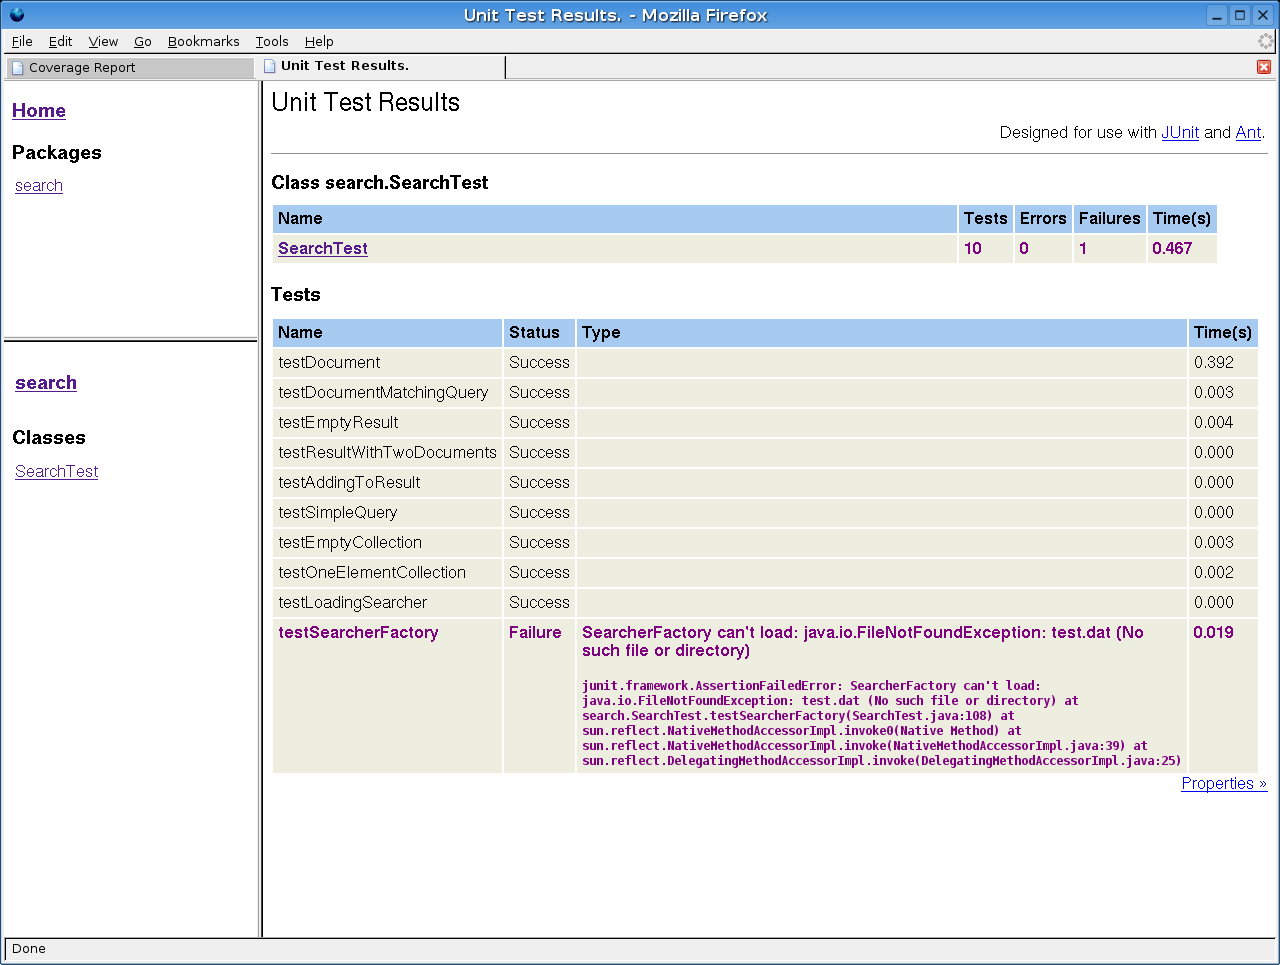
\includegraphics[width=0.75\linewidth]{qm/junitreport}
\end{center}
\else
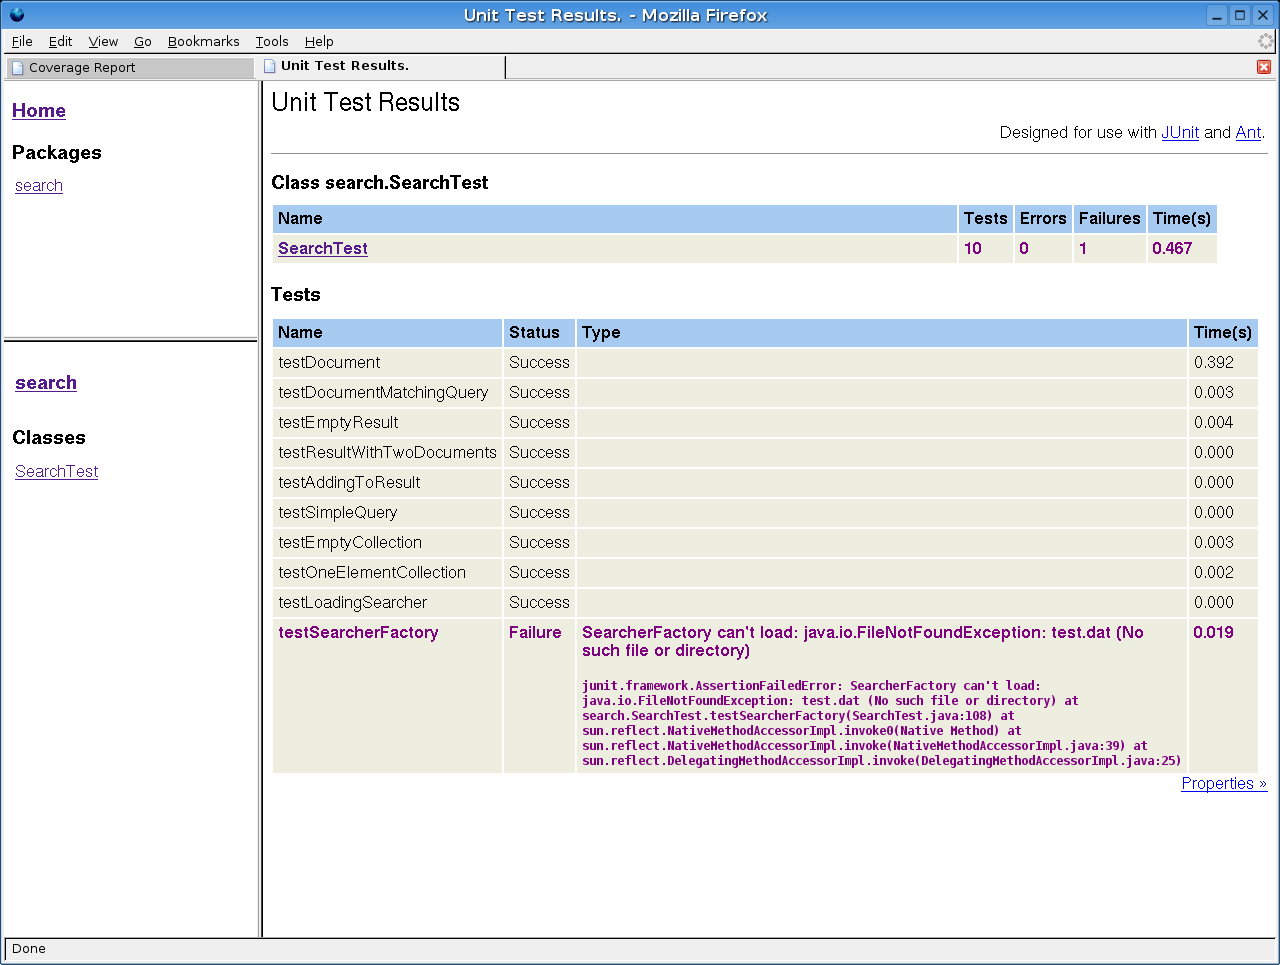
\includegraphics[width=\linewidth]{qm/junitreport}
\fi
\caption{Ein mit Apache Ant erzeugter Junit-Report}
\end{figure}
%HINWEIS: Problem bei Eclipse. (www.ryanlowe.ca)
%
%  ``.. Ant could not find the task or a class this task relies upon ..''
%
% .. So you need to tell Ant where to find a copy of junit.jar:
%
%  Window $\longrightarrow$ Preferences, Ant $\longrightarrow$ Runtime
%
%  In the Classpath tab click on Global Entries and then Add External JARs....
%
% Eclipse already has a copy of JUnit, so in the dialog find your Eclipse
% plugins directory ([ECLIPSE\_DIR]/plugins/) and go to the JUnit plugin
% (presently org.junit\_3.8.1) and select junit.jar.
%
%%Now all of your Ant
%% scripts will know how to do the <junit> Ant task.
%%
%% www.cengua.com/clover
%%
\newslide
Mit Maven ist es wesentlich einfacher:
\begin{lstlisting}[language=xml,
  morekeywords={reporting,plugins,plugin,artifactId}]
<reporting>
  <plugins>
    <plugin>
      <artifactId>maven-surefire-plugin</artifactId>
      <version>2.22.2</version>
    </plugin>
  </plugins>
</reporting>
\end{lstlisting}
Bemerkung: in Multimodul-Projekten kann mit
\lstinline[language=xml]{<aggregate>true</aggregate>}
dafür gesorgt werden, dass im
Parent-Modul die Resports aller Child-Module zusammengeführt werden.
%
\newslide
\subsection{Messung des Abdeckungsgrades}
Mit Code-Coverage-Analysen können ungetestete Code-Stellen identifiziert
werden. Dadurch lassen sich gezielt zusätzliche Unit-Tests entwickeln.

Man unterscheidet:

\begin{tabularx}{\linewidth}{l|X}
Typ            & Verhältnis \\
\hline
{\textbf Statement Coverage} (Line Coverage) & Anzahl ausgeführte zu
  vorhandene Anweisungen\\
{\textbf Branch Coverage} & Anzahl ausgeführte zu vorhandene Verzweigungen\\
{\textbf Condition Coverage} & Anzahl ausgeführte zu vorhandene
Fallunterscheidungen \\
{\textbf Function Coverage} & Anzahl ausgeführte zu vorhandene Funktionen\\
\end{tabularx}

\newslide
Um die Messungen durchführen zu können, muss der Code entsprechend angepasst,
oder ``instrumentiert'' werden. Dies kann grundsätzlich auf der Source-Code-
oder (bei Java) auf der Byte-Code-Ebene geschehen. Das Open-Source-Werkzeug
Cobertura fügt den notwendigen Code in den Byte-Code der Class-Dateien.
Es kann auf mehrere Arten aufgerufen werden:
von der Kommandozeile, mit Ant oder Maven.

\newslide
Bei Ant ist der Ausgangspunkt ist die Build-Datei, die wie folgt erstellt wird:
\begin{enumerate}
\item Man deklariert die Cobertura-Tasks \verb+cobertura-instrument+ und
  \verb+cobertura-report+:
  \begin{lstlisting}[language=xml,morekeywords={taskdef}]
<taskdef classpath="cobertura.jar" resource="task.properties" />
  \end{lstlisting}
\newslide
\item Man sorgt dafür, dass die Class-Dateien instrumentiert werden:
  \begin{lstlisting}[language=xml,
    morekeywords={cobertura,instrument,fileset,include,exclude}]
<cobertura-instrument todir="instrument">
   <fileset dir="build">
      <include name="**/*.class" />
      <exclude name="**/*Test.class" />
   </fileset>
</cobertura-instrument>
  \end{lstlisting}
  Damit werden die angepassten Dateien ins Verzeichnis intrument abgelegt.
\newslide
\item Bei der Test-Durchführung müssen neu die geänderten Dateien verwendet
  werden:
  \begin{lstlisting}[language=xml,morekeywords={junit,classpath}]
<junit fork="yes" printsummary="true">
  <classpath location="instrument" />
  <classpath location="build" />
  ...
</junit>
  \end{lstlisting}
  Ausserdem muss das Attribut fork auf yes gesetzt werden.
\newslide
\item Anschliessend wird ein Report in HTML-Format erstellt:
  \begin{lstlisting}[language=xml,morekeywords={cobertura,report}]
<cobertura-report srcdir="src" destdir="coverage/html"/>
  \end{lstlisting}
\end{enumerate}
%
Mit Maven ist es auch hier wesentlich einfacher:
\begin{lstlisting}[language=xml,
  morekeywords={reporting,plugins,plugin,groupId,artifactId}]
  <reporting>
    <plugins>
      <plugin>
        <groupId>org.codehaus.mojo</groupId>
        <artifactId>cobertura-maven-plugin</artifactId>
      </plugin>
    </plugins>
  </reporting>
\end{lstlisting}
\ifslides
  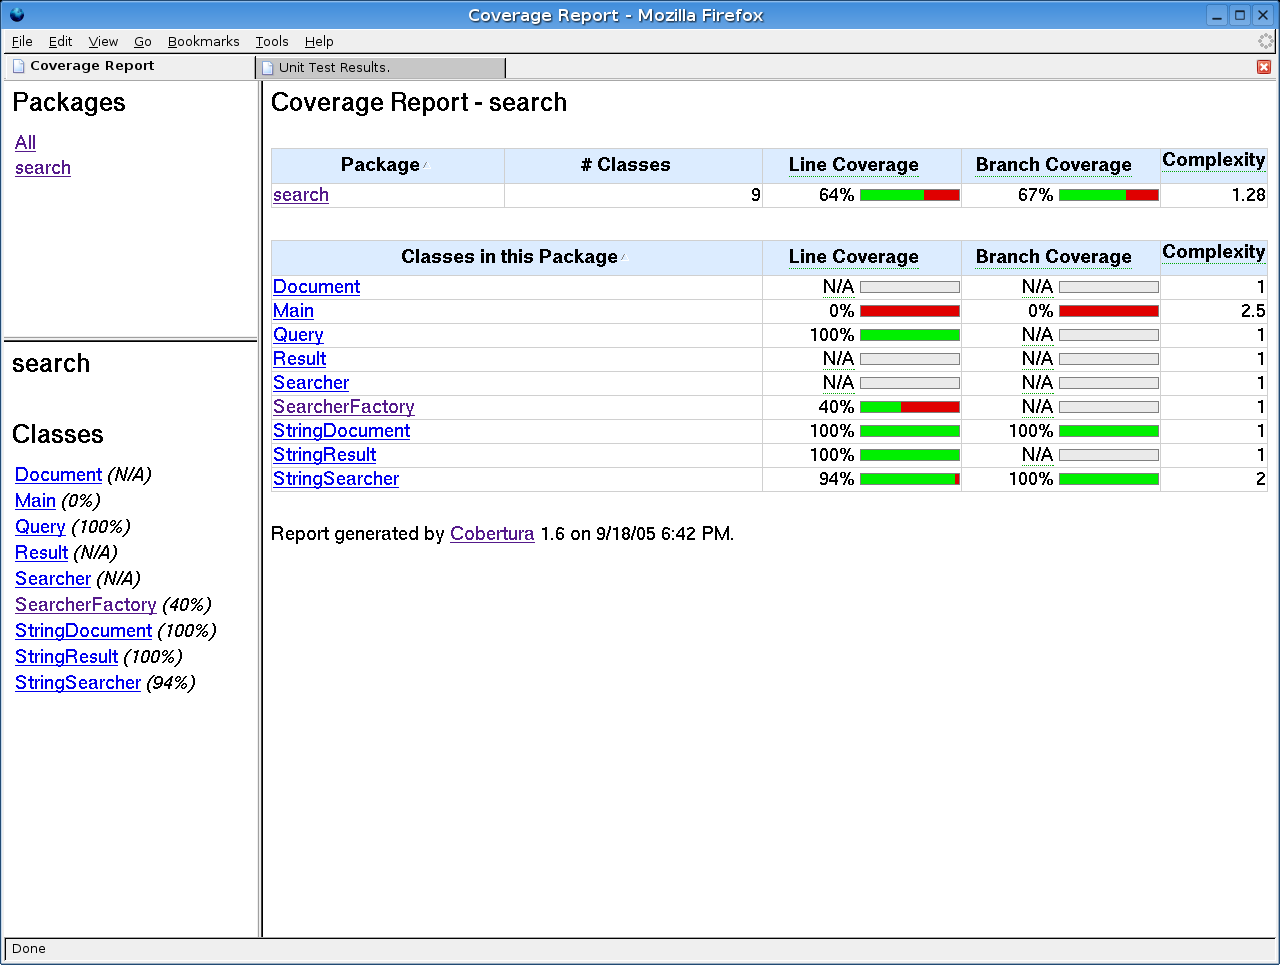
\includegraphics[width=0.9\linewidth]{qm/coverage}
\else
\begin{figure}[H]
  \centering
  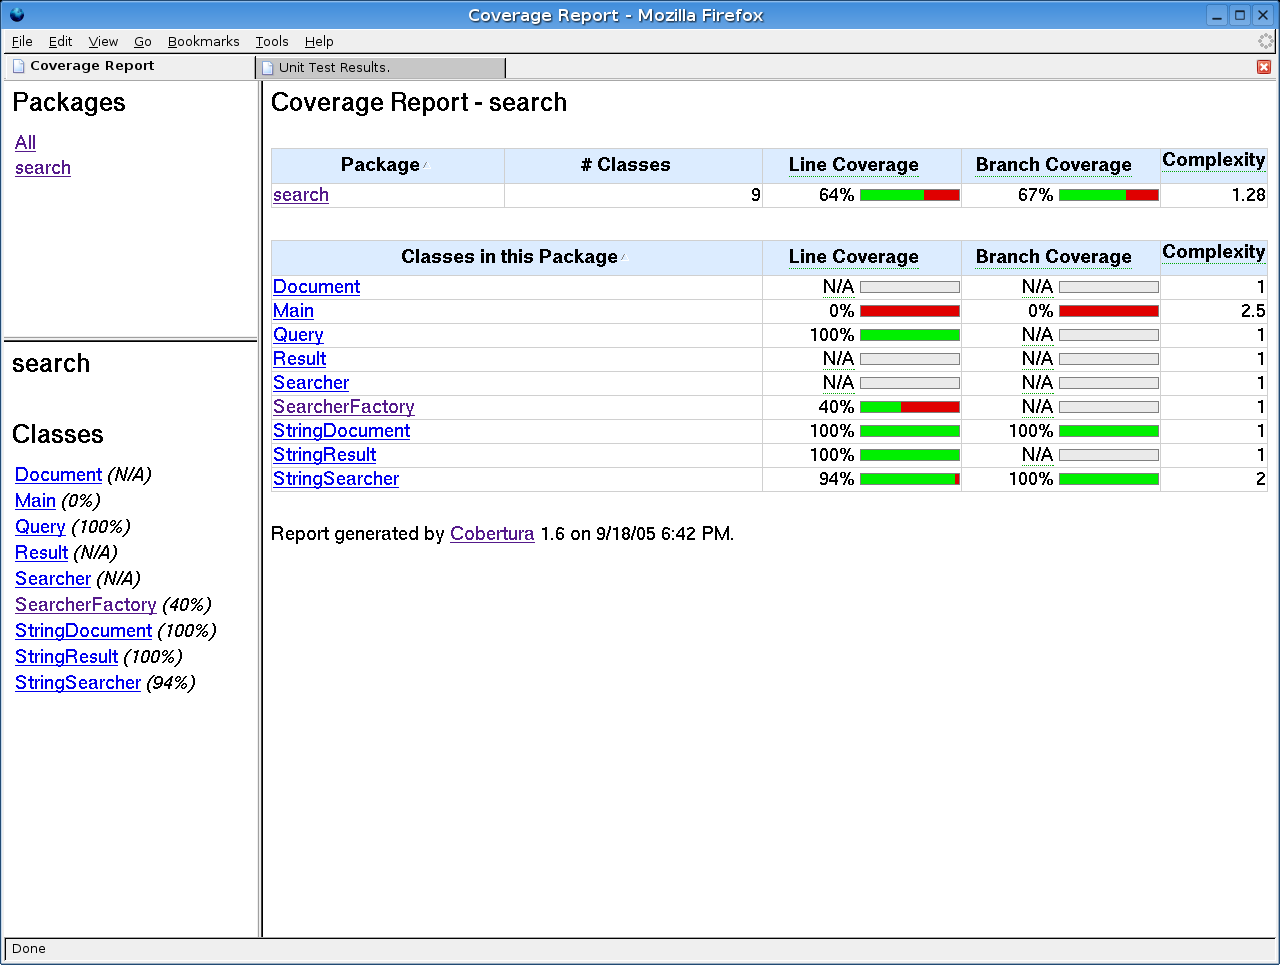
\includegraphics[width=\linewidth]{qm/coverage}
  \caption{Test-Coverage Report mit Cobertura}
  \label{fig:cobertura}
\end{figure}
\fi
%-------------------------------------------------------------------------
\newpage

\section{Continuous Integration}
\emph{Don’t break the nightly build!}
is a cardinal rule in software development shops that post a
freshly built daily product version every morning for their testers.

\vspace{3mm}

Continuous Integration is a software development practice in which
developers are required to frequently commit changes to the
source code in a shared repository. Each commit is then continuously
pulled and built.\\
The goal of Continuous Integration is to provide rapid feedback so that if
a defect is introduced into the code base, it can be identified and
corrected as soon as possible.\\
That approach will ensure that:

%Mit dem Begriff ``Continuous Integration'' (abgekürzt CI) bezeichnet man das
%automatisierte, regelmässige und häufige Erstellen eines Softwaresystems während
%dessen Entwicklung. Damit kann auf einfachste Weise sichergestellt
%werden, dass

\begin{itemize}
%\item allfällige Integrationsprobleme frühzeitig erkannt,
\item identify defects as soon as possible
%\item alle benötigten Dateien eingecheckt und
\item all sources are in the repository to build the system
%\item die vorhandenen Tests durchgeführt worden sind.
\item all available tests are executed successfully
\end{itemize}

Important are frequent commit and push operations. Working
many days in a row without pushing the results into the repository will
increase the probability that something will fail.\\
A CI server ensures, that new code in the repository will
directly be included in the build process.\\
It is also possible to sent out mail notifications in case of
a successful build.\\
This process is also called \emph{Smoke Testing}.
Smoke Testing is a software testing process that determines whether
the deployed software build is stable or not. Smoke testing is a
confirmation for QA team to proceed with further software testing.
It consists of a minimal set of tests run on each build to test
software functionalities.
%Dieses Verfahren wird auch ``Smoke Testing'' genannt, in
%Anlehnung an das Vorgehen bei der Hardware-Entwicklung, wenn nach
%erfolgter Bestückung einer Platine Spannung angelegt wird um
%festzustellen, ob irgendwo Rauch aufsteigt.

Available continuous integration systems:
\begin{itemize}
\item CruiseControl \href{http://cruisecontrol.sourceforge.net}
                        {cruisecontrol.sourceforge.net}
\item Jenkins/Hudson \href{http://jenkins-ci.org}{jenkins-ci.org}
\item Bamboo  \href{http://www.atlassian.com/software/bamboo}
     {www.atlassian.com/software/bamboo}
\item Continuum \href{http://continuum.apache.org}{continuum.apache.org}
\item TeamCity  \href{http://www.jetbrains.com/teamcity}
      {www.jetbrains.com/teamcity}
\item GitLab \href{http://www.gitlab.com}
      {www.gitlab.com}
%\item \ldots
\end{itemize}
%
\newslide
\subsection{Jenkins}
Jenkins offers a simple way to set up a continuous integration or
continuous delivery (CI/CD) environment for almost any combination
of languages and source code repositories using pipelines,
as well as automating other routine development tasks.
While Jenkins doesn’t eliminate the need to create scripts for
individual steps, it does give you a faster and more robust way to
integrate your entire chain of build, test, and deployment tools
than you can easily build yourself.\\
Jenins will be installed as a server component. You could deploy it as
a web application (e.g. Tomcat, JBoss) or run it with the integrated
server.\\
The configuration of the system and the build processes are set up by
using the web front end application.

\begin{figure}[H]
  \centering
  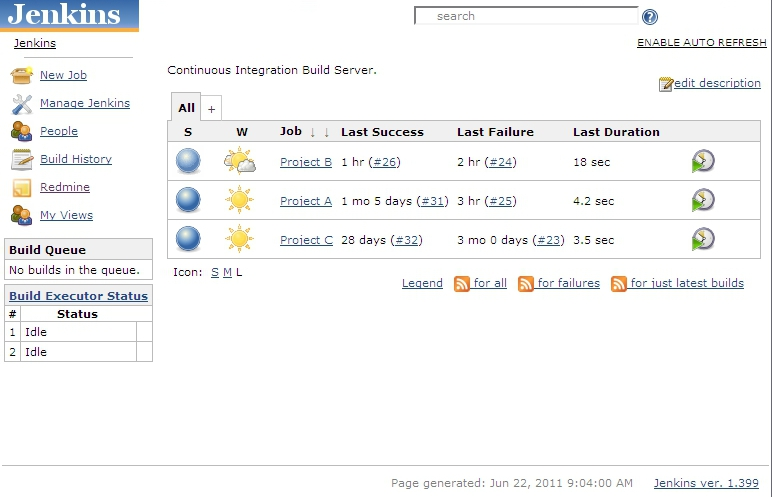
\includegraphics[width=0.8\linewidth]{qm/jenkins}
  \caption{Jenkins GUI (Quelle: J. Ferguson Smart)}
  \label{fig:jenkins}
\end{figure}

In addition, there is a REST interface and a command line tool
available.

\vspace{3mm}

Jenkins unterscheidet die folgenden Projekt-Typen:
\begin{itemize}
\item Free-Style-Projekt: ausführen von Funktionen, die in Shell-,
  Windows Batch- oder Ant-Skripts enthalten sind,
\item Maven-2-Projekt: Durchführung eines Maven-Build-Prozesses,
\item Multikonfigurationsprojekt: mehrfache Durchführung
  eines Builds für unterschiedliche Konfigurationen (Matrix-Build).
\end{itemize}
Die Auslösung eines Build-Vorganges kann auf verschiedene Weise
geschehen:
\begin{itemize}
\item nachdem ein Build-Vorgang beendet ist,
\item in periodischen Intervallen: MIN HOUR DOM MONTH DOW
\item bei Änderungen im SCM
\item explizit
\end{itemize}
% John Ferguson Smart
%\href{http://www.wakaleo.com/public_resources/continuous-integration-with-hudson.pdf}
%\newslide
%\subsection{Aufgabe}
%Ein Maven-basiertes Projekt soll von einem CI-Server überwacht
%werden.
%Nehmen Sie ein geeignetes System in Betrieb und sorgen Sie dafür,
%dass die Junit- und Checkstyle-Reports nach einem Build jeweils
%angezeigt werden.
%
%Tipp:
%\href{http://cruisecontrol.sourceforge.net/gettingstartedsourcedist.html#Modifying_the_HTML_Reports}{cruisecontrol.sourceforge.net/gettingstartedsourcedist.html\#Modifying\_the\_HTML\_Reports}
%
%\newpage
\newslide

\section{Memory Tests}
It is important to know the memory consumption behavior of the
software system. Especially to find out if there are any memory leaks.\\
A memory leak is a type of resource leak that occurs when a computer
program incorrectly manages memory allocations in a way that memory which
is no longer needed is not released. After a specific amount of time,
the system will crash with a memory exception.\\
A hint for a memory leak is the increase of memory usage over time.\\
There are several tools available to check for memory usage. Default
tools are:

\begin{itemize}
\item Windows: Task Manager
\item Linux/OSX: Top
\end{itemize}

\begin{figure}[H]
  \centering
  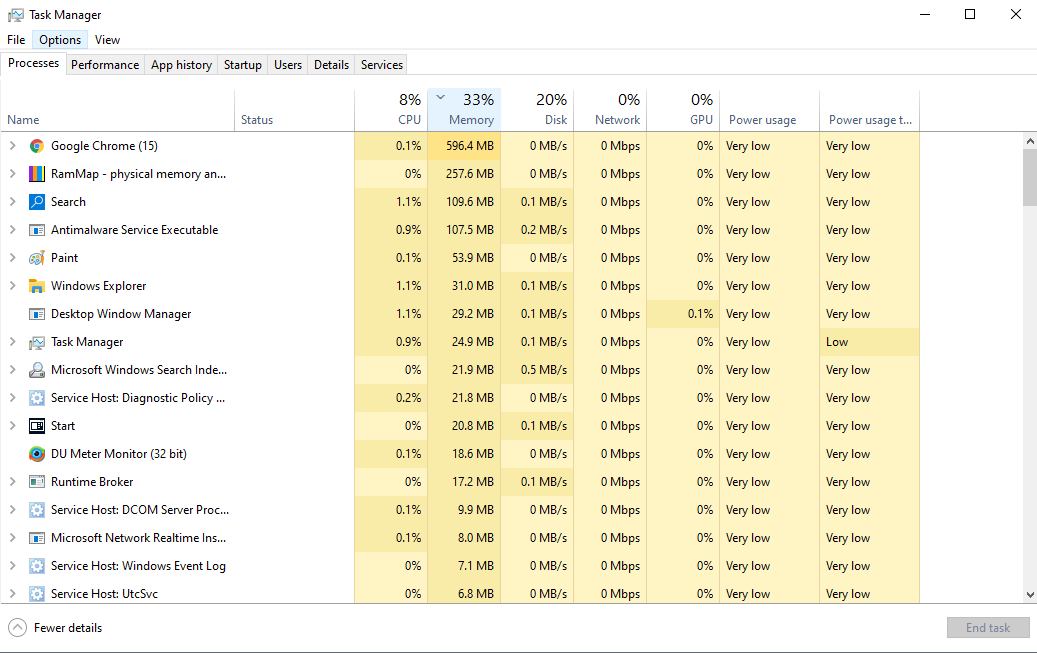
\includegraphics[width=0.8\linewidth]{qm/taskmanager}
  \caption{Windows Task Manager}
\end{figure}

\vspace{3mm}

\begin{figure}[H]
  \centering
  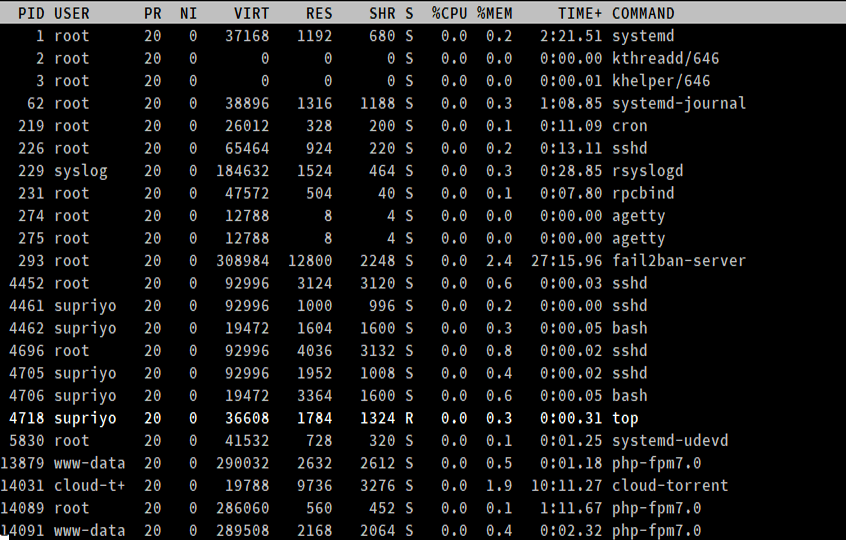
\includegraphics[width=0.8\linewidth]{qm/topcmd}
  \caption{top command}
\end{figure}

\section{Zulu Mission Control}
Zulu Mission Control is a build of JDK Mission Control,
an open source Java runtime profiling and monitoring utility
originally developed by JRockit and open source by Oracle in 2018.
JDK Mission control was originally developed for Java 11,
and Azul Systems has back-ported the utility to also support
properly-configured builds of OpenJDK 8.

\vspace{3mm}

Zulu Mission Control will detect a running Java application and
will be able to hook up with Java application.

\begin{figure}[H]
  \centering
  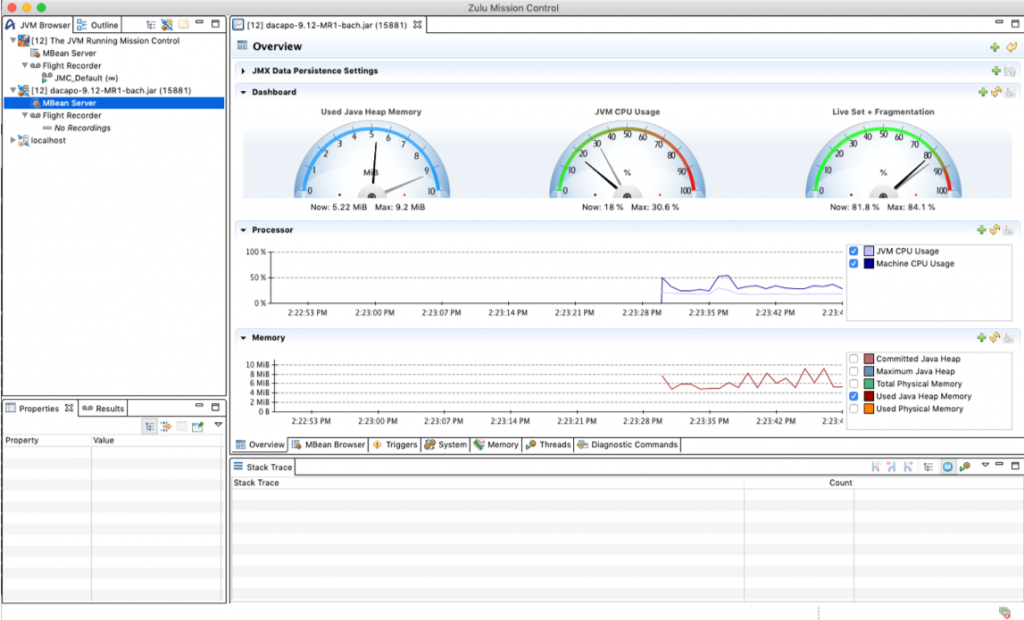
\includegraphics[width=0.8\linewidth]{qm/zmc}
  \caption{Zulu Mission Control}
\end{figure}




https://www.azul.com/products/zulu-mission-control/

\section{Speichertests mit Valgrind}
Valgrind ist ein Open-Source-Tool für das Auffinden von
Speicher-Managementproblemen in Linux-x86-Programmen:
\begin{itemize}
\item nicht-initialisierter Speicher
\item Zugriffe auf bereits freigegebenen Speicher
\item Bereichsüberschreitungen
\item nicht freigegebener Speicher
\item Unkorrekte Verwendung von malloc/new/new[] versus free/delete/delete[]
\end{itemize}
Valgrind hat den ``Open Source Award 2004'' gewonnen und wird im
KDE-Projekt ausgiebig eingesetzt. Der Gebrauch ist recht einfach. Valgrind
wird einfach beim Aufstarten des  zu testenden Programmes auf der
Kommandozeile vor den Programmnamen gesetzt:
\begin{verbatim}
linux> valgrind --tool=memcheck ./mein_program
\end{verbatim}
Beispiel:
{
\ifslides\footnotesize
\else\small
\fi
\begin{verbatim}
==15506== Memcheck, a memory error detector for x86-linux.
==15506== Copyright (C) 2002-2004, and GNU GPL'd, by Julian Seward et al.
==15506== Using valgrind-2.2.0, a program supervision framework for x86-linux.
==15506== Copyright (C) 2000-2004, and GNU GPL'd, by Julian Seward et al.
==15506== For more details, rerun with: -v
==15506==
==15506== Invalid write of size 1
==15506==    at 0x8048AED: Sstring::Sstring(char const*) (my_prog.cc:8)
==15506==    by 0x804885D: main (my_prog.cc:29)
==15506==  Address 0x1BB3F046 is 0 bytes after a block of size 30 alloc'd
==15506==    at 0x1B9071D5: operator new[](unsigned) (vg_replace_malloc.c:139)
==15506==    by 0x8048ABF: Sstring::Sstring(char const*) (my_prog.cc:7)
==15506==    by 0x804885D: main (my_prog.cc:29)
..
\end{verbatim}
}
\ifslides
\else
Die Zahl zwischen den beiden Gleichheitszeichen bezeichnet die Prozessnummer.
\fi
%
\newpage
\section{GUI-Tests mit Abbot und FEST}
Das Testen von grafischen Benutzeroberflächen
ist meist eine heikle Angelegenheit. Hauptsächlich hat dies
damit zu tun, dass bereits kleine Layout-Änderungen bei
automatisierten Tests zu unerwarteten Störungen führen können.
Teilweise kann dies zwar umgangen werden,
indem man Layout-bezogene Tests nach Möglichkeit vermeidet. Trotzdem, auf
händisch durchgeführte Tests kann bei GUI-Tests meist nicht verzichtet werden.

\newslide
Man unterscheidet grundsätzlich zwei Verfahren:
\begin{enumerate}
\item GUI-Unit-Tests: Tests werden entwickelt, bevor GUI-Code
  vorhanden ist. Beispiel:
\begin{lstlisting}[language=java]
public class CelsiusConverterTest extends TestCase {
  public void testConversion(){
    CelsiusConverter conv = new CelsiusConverter();
    conv.tempCelsius.setText("35");
    conv.convertTemp.doClick();
    assertEquals(conv.fahrenheitLabel.getText(),"95 Fahrenheit");
  }
}
\end{lstlisting}
\newslide
\item Record/Playback (Capture/Replay): bestimmte Bedienungsabläufe werden
in Skriptform aufgezeichnet. Danach wird das Skript
an ausgewählten Stellen mit Testbedingungen ergänzt. Die
Testdurchführung kann damit automatisiert ablaufen.
\end{enumerate}
\begin{minipage}{0.48\linewidth}
\ifslides
\else
Beispiel Abbot:
\fi
\begin{enumerate}
\item Starten des Script-Editors Costello:
\begin{lstlisting}
  % java -jar lib/costello.jar
\end{lstlisting}
\item Ein neues Skript erstellen:

  File $\longrightarrow$ New Script
\item Eingabe der ``Launch''-Information:

\begin{tabular}{ll}
  Target Class Name & CelsiusConverter\\
  method & main \\
  Arguments & \verb+[]+\\
 Classpath & \\
\end{tabular}
\item Starten der Test-Applikation:

   Test $\longrightarrow$ Launch
\item Beginn der Aufzeichnung:

  Capture $\longrightarrow$ All Actions
\setcounter{saveenum}{\value{enumi}}
\end{enumerate}
\end{minipage}
\begin{minipage}{0.5\linewidth}
\begin{figure}[H]
\begin{center}
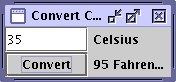
\includegraphics[width=0.4\linewidth]{qm/celsius}
\end{center}
\vspace{1cm}

\hfill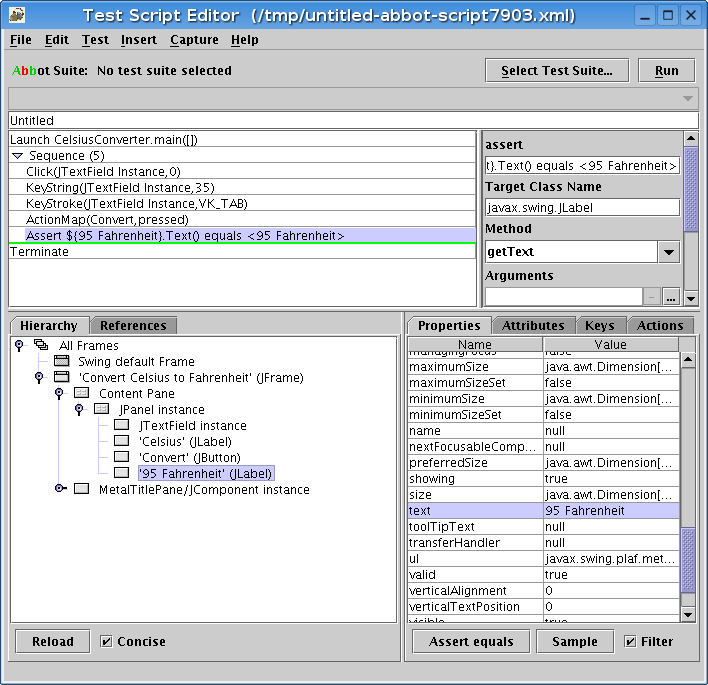
\includegraphics[width=0.9\linewidth]{qm/abbot}\\
\caption{GUI-Test mit Abbot}
\end{figure}
\end{minipage}

\begin{enumerate}
\setcounter{enumi}{\value{saveenum}}
\item Den Wert ``35'' im CelsiusConverter-Dialog eingeben und anschliessend
  ``Convert'' aktivieren.
\item Die Zeile ``ActionMap(Convert,pressed)'' selektieren.
\item Im Hierarchy-Fenster den Eintrag ``95 Fahrenheit (JLabel)'' selektieren.
\item Im Properties-Fenster die Zeile ``text  95 Fahrenheit'' selektieren.
\item Den Button ``Assert equals'' aktivieren.
\item Ausführen des Tests: ``Run'' aktivieren.
\item Script abspeichern: File $\longrightarrow$ Save as \ldots
\item Filename ``CelsiusConverterTest.xml'' eingeben.
\item Test ausführen:
  \begin{lstlisting}
  % java -cp lib/costello.jar junit.extensions.abbot.ScriptFixture \
       CelsiusConverterTest.xml
  \end{lstlisting}
\end{enumerate}
%
Das Projekt
FEST-Swing
(Fixtures for Easy Software Testing) stellt aufbauend auf Abbot
ein API zur Verfügung, welches das Erstellen und Pflegen von GUI-Tests
vereinfacht. Es zeichnet sich durch die folgenden Eigenschaften aus:
\begin{enumerate}
  \item Simulation
  der Benutzereingaben (Mauszeiger- und Tastatur-Ereignisse),
  \item robuster Zugriff auf GUI-Komponenten mittels verschiedener
    Suchverfahren: nach Typ, Name oder nach benutzerdefinierten Kriterien,
  \item Unterstützung sämtlicher Swing-Komponenten der JDK,
  \item kompaktes und leistungsfähiges API für die Erstellung und
    Anpassung funktionaler GUI-Tests,
  \item Möglichkeit Dialogabbildungen fehlgeschlagener Tests in die
  Testreports einzubinden,
  \item kann sowohl mit JUnit wie auch TestNG verwendet werden.
  \end{enumerate}
Beispiel:
  \begin{lstlisting}[language=java]
public class FestSearchTest extends TestCase {
  private FrameFixture window;

  public void setUp(){
    SearchPanel sp = new SearchPanel();
    JFrame dialog = new JFrame("Bibliographic System - TEST");
    dialog.getContentPane().add(sp);
    window = new FrameFixture(dialog);
    window.show();
  }

  public void tearDown() {
    window.cleanUp();
  }

  public void testSearch(){
    window.textBox("queryField").enterText("a");
    window.button("findButton").click();
    window.textBox("queryField").requireText("a");
  }
}
\end{lstlisting}
%
%\subsection{Aufgabe}
%Führen Sie die notwendigen Anpassungen durch,
%so dass mit der Klasse FestSearchTest getestet
%werden kann, ob die Tabelle resultTable des Search-Dialogfensters
%nach einer Such-Abfrage die korrekten
%Einträge anzeigt.
%
\newpage
TODO: Include WEBTEST
\newpage
\subsection{Testen von Web-Applikationen}
%Die Integration des Testens in die Software-Entwicklung ist auch bei
%Web-Applikationen sehr zu empfehlen. Modifikationen und Erweiterungen können
%so einfacher durchgeführt werden, da man weniger Gefahr läuft, dass als Folge
%davon plötzlich unerwartete Störungen auftreten. Ein gut konfiguriertes
%Testsystem ist in der Lage derartige Probleme frühzeitig aufzudecken.
%
%\newslide
Für das automatisierte Testen von Web-Applikationen
stehen eine Reihe frei-erhältlicher Tools zur Verfügung:
\begin{itemize}
%\item Cactus: das Test-Framework des Apache-Jakarta-Projektes für Unit-Tests
%  von server-seitigem Code (Servlets, Filters, Tag Libs, EJB \ldots)
%\href{http://jakarta.apache.org/cactus}{jakarta.apache.org/cactus}
\item HtmlUnit: automatisierter Funkionstest von Web-Seiten mit JavaScript,
  Cookies, Authentication und Page Redirection
\href{http://htmlunit.sourceforge.net/}{htmlunit.sourceforge.net}
\item JWebUnit: Durchführung von Abnahmetests
\href{http://jwebunit.sourceforge.net/}{jwebunit.sourceforge.net/}
\item MaxQ: Python-basiertes Aufnahme/Wiedergabe-Tool
\href{http://maxq.tigris.org/}{maxq.tigris.org/}
\item Canoo WebTest:

\href{http://webtest.canoo.com/webtest/manual/WebTestHome.html}
{webtest.canoo.com/webtest/manual/WebTestHome.html}
\item Selenium:
\href{http://selenium.openqa.org}{selenium.openqa.org}
\item Cargo: ein Wrapper für Java-EE-Container
 \href{http://cargo.codehaus.org/Home}{cargo.codehaus.org/Home}
\item JMeter: Durchführung von Lasttests
\href{http://jakarta.apache.org/jmeter}{jakarta.apache.org/jmeter}
\item Grinder: Durchführung von Lasttests mit Jython-Scripts
  \href{http://grinder.sourceforge.net}{grinder.sourceforge.net}
\end{itemize}
\newslide
\subsubsection{HtmlUnit}
HtmlUnit wird als ``Browser für Java-Programme'' bezeichnet.
HtmlUnit basiert auf Junit. Das heisst, man geht grundsätzlich wie gewohnt vor:
Man erstellt eine Testklasse und fügt
 dieser Klasse
 sukzessive die entsprechenden Testmethoden hinzu. 

\newslide
Am einfachsten verwendet man 
HtmlUnit mit Maven und ergänzt das POM-File mit folgendem Element:
\begin{lstlisting}[language=xml,
   morekeywords={dependency,groupId,artifactId,version,scope}]
<dependency>
  <groupId>net.sourceforge.htmlunit</groupId>
  <artifactId>htmlunit</artifactId>
  <version>2.4</version>
</dependency>
\end{lstlisting}
Dazu muss die Junit-Version auf den Wert 4.4 gesetzt werden.
\newslide
Als Testfall 
wird man in der Regel eine Server-Verbindung kreieren und überprüfen, ob die
erwarteten Ergebnisse zurückgegeben werden:
\begin{lstlisting}[language=java]
public class SimpleWebTest {
  @Test
  public void homePage() throws Exception {
    final WebClient webClient = new WebClient();
    final HtmlPage page = (HtmlPage)webClient.
                 getPage("http://localhost:8080/hitchhikers-guide");
    assertEquals("Welcome", page.getTitleText());
  }
\end{lstlisting}
\newslide
Das folgende Beispiel zeigt, dass auch Web-Formulare getestet werden können:
\begin{lstlisting}[language=java]
  @Test
  public void submitForm() throws Exception {
    final WebClient webClient = new WebClient();
    final HtmlPage page1 = (HtmlPage)webClient.
                 getPage("http://localhost:8080/hello/login");
    final HtmlForm page1.getFormByName("loginform");
    final HtmlTextInput textfield = form.getInputByName("username");
    final HtmlSubmitInput button = form.getInputByName("submit");

    textfield.setValueAttribute("douglas");
    final HtmlPage page2=(HtmlPage)button.click();
    assertEquals( "Main", page.getTitleText() );
  }
\end{lstlisting}

\newslide
\subsubsection{JWebUnit}
JWebUnit ist ein auf Junit und HtmlUnit basierendes
Java-Test-Framework für Web-Applikationen. JWebUnit verwendet man am
einfachsten mit Maven:
\begin{lstlisting}[language=xml,
  morekeywords={dependency,groupId,artifactId,version,scope}]
<dependency>
  <groupId>net.sourceforge.jwebunit</groupId>
  <artifactId>jwebunit-htmlunit-plugin</artifactId>
  <version>2.2</version>
  <scope>test</scope>
</dependency>
 \end{lstlisting}
\newslide
Im Vergleich zu HtmlUnit ist die Verwendung einfacher:
\begin{lstlisting}[language=java]
public class SimpleWebUnitWebTest extends WebTestCase {
  public void setUp(){
    getTestContext().
         setBaseUrl("http://localhost:8080/hitchhiker");
  }
  public void testHomePage() {
    beginAt("/");
    assertTitleEquals("Welcome");
  }
}
\end{lstlisting}
\newslide
Das gilt auch für Formulare:
\begin{lstlisting}[language=java]

  public void testSubmitForm() throws Exception {
    beginAt("/hello/login");
    assertFormPresent("loginform");
    assertFormElementPresent("username");
    setTextField("username", "douglas");
    submit();
    assertTitleEquals( "Main" );
  }
\end{lstlisting}
\newslide
Weitere Vereinfachungen betreffen das Testen von Tabellen und HTML-Elementen
und das Navigieren durch die Seiten.
\begin{lstlisting}[language=java]
  assertElementPresent("pageTitle");
  assertTextInElement("pageTitle", "Hello World");
\end{lstlisting}
In diesem Beispiel wird geprüft, ob ein Element
mit dem Id-Attribut ``pageTitle'' existiert und ob darin der
Text ``Hello World'' enthalten ist.

\newslide
Störend ist hier wie schon bei HtmlUnit, 
dass zuerst ein WebContainer gestartet
werden muss, bevor man die Tests durchführt.

\newslide
Dank Jetty können diese Tests aber wie normale Unit-Tests durchgeführt
werden:
\begin{lstlisting}[language=java]
import org.mortbay.jetty.Server;
public class SimpleWebUnitWebTest extends WebTestCase {
  private Server server;
	
  public void setUp() throws Exception{
    String context="/hitchhiker";
    // Port 0 means "assign arbitrarily port number"
    server = new Server(0);
    server.addHandler(new WebAppContext("src/main/webapp", context));
    server.start();
    int port = server.getConnectors()[0].getLocalPort();
    getTestContext().setBaseUrl("http://localhost:"+port+context);
  }
..
}
\end{lstlisting}
\newslide
Dazu muss lediglich die POM-Datei etwas angepasst werden:
\begin{lstlisting}[language=xml,
  morekeywords={dependency,groupId,artifactId,version,scope}]
    <dependency>
      <groupId>org.mortbay.jetty</groupId>
      <artifactId>jetty</artifactId>
      <version>6.1.14</version>
      <scope>test</scope>
    </dependency>
    <dependency>
      <groupId>org.mortbay.jetty</groupId>
      <artifactId>jsp-2.1</artifactId>
      <version>6.1.14</version>
      <scope>test</scope>
    </dependency> 
\end{lstlisting}
\newslide
% http://blog.bemoko.com/2009/07/01/automated-mobile-web-testing-with-canoo-webtest-were-impressed/
%
\subsubsection{Canoo WebTest}
Auch Canoo WebTest ist ein auf HtmlUnit basierendes
Java-Test-Framework für Web-Applikationen. Im Gegensatz zu JWebUnit
werden die Testfälle jedoch als Ant-Tasks definiert:
\begin{lstlisting}[language=xml,
  morekeywords={project,property,import,target,webtest,config,steps,invoke,verifyTitle,setInputField,clickButton,verifyTitle}]
<project name="SimpleTest" basedir="." default="wt.full">

  <property name="webtest.home"
            location="/usr/local/java/webtest-3.0" />
  <import file="${webtest.home}/webtest.xml"/>

    <!-- runs start page test -->
    <target name="wt.testInWork"
        description="executes start page test case">

      <webtest
         name="check that WebTest is Google's top result">
	<config summary="true" />
	<steps>
	  <invoke url="http://www.google.com/ncr"
		  description="Go to Google (in English)"/>
	  <verifyTitle text="Google" />
	  <setInputField name="q" value="WebTest" />
	  <clickButton label="I'm Feeling Lucky" />
	  <verifyTitle text="Canoo WebTest Homepage" />
	</steps>
      </webtest>
    </target>
</project>
\end{lstlisting}
Ausgeführt werden diese Tests mit der Anweisung:
\begin{lstlisting}
  webtest -f web-test.xml
\end{lstlisting}
Webtest ist auch in der Lage übersichtliche Testreports zu generieren:
\begin{figure}[H]
  \centering
  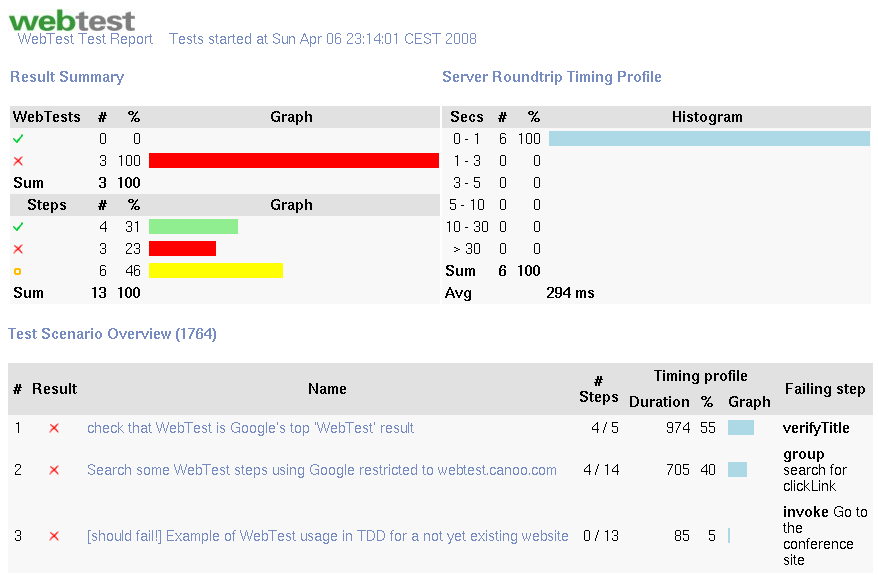
\includegraphics[width=0.8\linewidth]{qm/canoo-webtest-report}
  \caption{Canoo Webtest Report}
  \label{fig:canoo-webtest}
\end{figure}
Man kann Webtest auch in einem Maven-Projekt verwenden:
%allerdings muss zur Zeit das Plugin von Siegfrid Goeschl's Web-Seite
%
%\href{http://people.apache.org/~sgoeschl/download/maven-plugins/webtest-maven-plugin}
%  {people.apache.org/~sgoeschl/download/maven-plugins/webtest-maven-plugin}
%
%herunter geladen
% und eigenhändig im Maven-Repository installiert werden:
%
% Siehe:
% http://mguillem.wordpress.com/2009/04/30/webtest-with-groovy-maven-and-eclipse/
%
% ant -f /usr/local/java/webtest/webtest.xml wt.createProject
%
\begin{lstlisting}[language=xml,
  morekeywords={plugin,groupId,artifactId,configuration,host,port,haltonfailure,haltonerror,loglevel,executions,execution,phase,goals,goal}]
  <plugin>
    <groupId>org.codehaus.mojo</groupId>
    <artifactId>webtest-maven-plugin</artifactId>
    <configuration>
      <host>localhost</host>
      <port>8080</port>
    </configuration>
    <executions>
      <execution>
        <phase>integration-test</phase>
          <goals>
	    <goal>test</goal>
	  </goals>
	</execution>
      </executions>
  </plugin>
\end{lstlisting}
Das Plugin erwartet die webtest.xml-Datei im Verzeichnis
src/test/webtest.

Eine gutes Beispiel dazu findet man bei
Matt Raibles AppFuse-Framework \href{http://appfuse.org}{appfuse.org},
welches auch ganz allgemein beim Kick-Starting von Web-Projekten
ungemein nützlich ist.
%
% weitere beispiele:
%
% http://www.philliprhodes.com/content/testing-drupal-grails-webtest
% http://weblogs.java.net/blog/felipegaucho/archive/2009/11/18/testing-pdf-files-canoo-webtest-and-maven2
%
%
%\begin{lstlisting}[language=xml]
% <dependencies>
%     ...
%     <dependency>
%         <groupId>com.canoo.webtest</groupId>
%         <artifactId>webtest</artifactId>
%         <version>3.1-SNAPSHOT</version>
%     </dependency>
% </dependencies>
% ...
% <repositories>
%     <repository>
%         <id>webtest-dependencies-snapshot</id>
%         <name>WebTest dependencies</name>
%         <url>http://webtest.canoo.com/webtest/m2-repo-snapshots</url>
%     </repository>
% </repositories>
% \end{lstlisting}

\newslide
\subsubsection{Selenium}
Selenium ist ein OpenSource-Framework für Abnahme-, System und
Funktionstests von Web-Applikationen. Selenium kann auf
unterschiedliche Weise eingesetzt werden:
\begin{itemize}
\item in einem Browser: Selenium Core (unterschiedliche Browser)
  eventuell in Ergänzung mit Selenium IDE (Firefox)
\item als Proxy-Server: Selenium Remote Control (RC) für die Durchführung
  automatisierter Web-Tests in unterschiedlichen Programmiersprachen
  (Java, C\#, Perl, Python, Ruby)
\end{itemize}
\newslide
Beispielsweise in Kombination mit JUnit:
\begin{lstlisting}[language=java]
public class SeleniumWebTest extends TestCase {
  private DefaultSelenium selenium;

  public void setUp() throws Exception {
    super.setUp();
    selenium = new DefaultSelenium("localhost", 4444,
                                   "*firefox",
                                   "http://localhost:8080/");
    selenium.start();
  }

  public void tearDown() throws Exception {
    selenium.stop();
    super.tearDown();
  }

  public void testHelloWorld() throws Exception {
    try {
      selenium.open("http://localhost:8080/hitchhikers-guide");
      assertEquals("Hello World", selenium.getText("//h2"));
    } catch (SeleniumException ex) {
      fail(ex.getMessage());
      throw ex;
    }
  }
}
\end{lstlisting}
\newslide
In einem Maven-Projekt (genauer in einem von Maven verwalteten Projekt)
ergänzt man das POM-File mit dem folgenden Dependency-Element
\begin{lstlisting}[language=xml,
  morekeywords={dependency,groupId,artifactId,version,scope,enabled}]
<dependency>
   <groupId>
      org.openqa.selenium.client-drivers
   </groupId>
   <artifactId>selenium-java-client-driver</artifactId>
   <version>0.9.2</version>
   <scope>test</scope>
</dependency>
\end{lstlisting}
\newslide
Dazu wird ein spezielles Maven-Repository benötigt:
\begin{lstlisting}[language=xml,
  morekeywords={repositories,repository,id,name,url,layout,snapshots,releases}]
 <repositories>
        <repository>
            <id>openqa</id>
            <name>OpenQA Repository</name>
            <url>http://maven.openqa.org</url>
            <layout>default</layout>
            <snapshots>
                <enabled>false</enabled>
            </snapshots>
            <releases>
                <enabled>true</enabled>
            </releases>
        </repository>
  </repositories>
\end{lstlisting}
\newslide
sowie die beiden folgenden Plugins:
\begin{lstlisting}[language=xml,
  morekeywords={plugin,groupId,artifactId}]
<plugin>
 <groupId>org.codehaus.mojo</groupId>
 <artifactId>selenium-maven-plugin</artifactId>
</plugin>
<plugin>
  <groupId>org.mortbay.jetty</groupId>
  <artifactId>maven-jetty-plugin</artifactId>
</plugin>
\end{lstlisting}
\newslide
Nun kann in einem Terminal die Web-Applikation gestartet werden:
\begin{lstlisting}
  % mvn jetty:run
\end{lstlisting}
in einem zweiten Terminal der Selenium-Server:
\begin{lstlisting}
  % mvn selenium:start-server
\end{lstlisting}
und schliesslich in einem dritten Terminal der Test:
\begin{lstlisting}
  mvn test
\end{lstlisting}
Für weitere Vereinfachung siehe

\href{http://wiki.foochal.org/index.php/Maven_Selenium#Simple_selenium_java_unit_test}
{wiki.foochal.org/index.php/Maven\_Selenium\#Simple\_selenium\_java\_unit\_test}

und

\href{http://binil.wordpress.com/2006/12/08/automated-smoke-tests-with-selenium-cargo-testng-and-maven/}
{binil.wordpress.com/2006/12/08/automated-smoke-tests-with-selenium-cargo-testng-and-maven/}
%
\begin{figure}[H]
\begin{center}
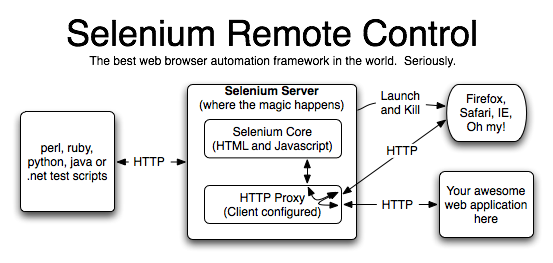
\includegraphics[width=\linewidth]{qm/selenium-rc}
\end{center}
\caption{Selenium Remote Control
  (Quelle \href{http://www.openqa.org/selenium-rc/tutorial.html}
   {www.openqa.org/selenium-rc/tutorial.html})}
\end{figure}
\begin{figure}[H]
\begin{center}
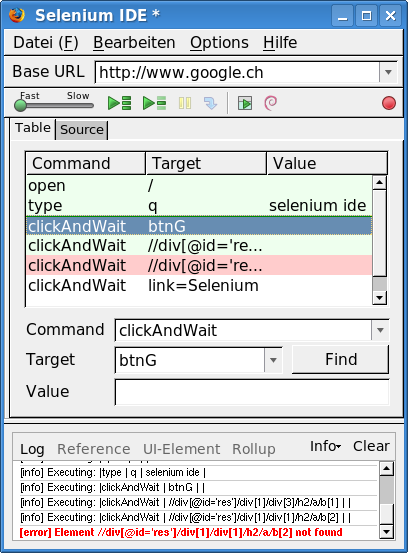
\includegraphics[width=0.5\linewidth]{qm/selenium-ide}
\end{center}
\caption{Selenium IDE als Firefox Plugin}
\end{figure}
%

%\subsection{Software und weitere Informationen}
%%% Local Variables:
%%% mode: latex
%%% TeX-master: "projektskizzen"
%%% End:

%
\section{Load tests with JMeter}
Mit JMeter, einem Java-basierten, Open-Source Tool aus dem
Apache/Jakarta-Projekt,  ist es möglich das Lastverhalten von
Client-Server-Applikationen zu testen.
%Nach dem Aufstarten von JMeter
%erscheint das folgende Dialogfenster:
%\begin{figure}[H]
%\includegraphics[width=\linewidth]{jmeter0}
%\caption{Dialogfenster von JMeter}
%\end{figure}

Als erstes erstellt man mit JMeter einen Testplan, der den Testablauf
beschreibt. Ein Testplan muss mindestens eine ``Thread Group'' enthalten.
Die Thread-Group bildet den Startpunkt des Testablaufes.
\begin{figure}[H]
\centering
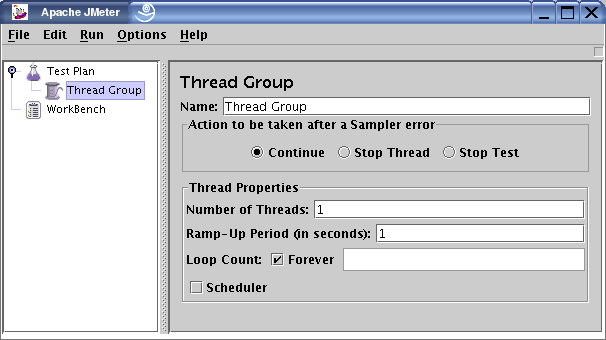
\includegraphics[width=0.7\linewidth]{qm/jmeter-threadgroup}
\caption{Dialogfenster von JMeter}
\end{figure}
\newslide
Eine Thread-Group enthält die folgenden Attribute:
\begin{itemize}
\item Name: der Name der Thread Group,
\item Number of Threads: jeder Thread entspricht einem einzelnen
  Benutzer,% Wenn man z.B. 10 Benutzer simulieren will, gibt man hier 10 ein.
\item Ramp-Up Period: Zeitdauer bis alle Threads erzeugt sind,
\item Loop Count: Anzahl Wiederholungen des Testablaufes (nur wenn nicht
  ``forever'')
\item Scheduler: hier können zusätzliche Parameter zur zeitlichen Steuerung des
  Tests eingegeben werden.
\end{itemize}
Nun kann man die weiteren Elemente eingeben, zum Beispiel Logic Controllers zur
Steuerung des Ablaufes, Samplers für die Erzeugung von Anfragen, Timers für
die zeitliche Verzögerung zweier aufeinanderfolgender Anfragen etc.

\newslide
Die folgende Liste zeigt ein Beispiel eines JMeter-Testplanes:
\begin{itemize}
\item Thread Group
  \begin{itemize}
    \item Once Only Controller
      \begin{itemize}
        \item Login Request (an HTTP Request )
      \end{itemize}
      \item Load Search Page (HTTP Sampler)
      \item Interleave Controller
      \begin{itemize}
        \item Search ``A'' (HTTP Sampler)
        \item Search ``B'' (HTTP Sampler)
        \item HTTP default request (Configuration Element)
      \end{itemize}
      \item HTTP default request (Configuration Element)
      \item Cookie Manager (Configuration Element)
      \item Graph results (Listener Element)
  \end{itemize}
\end{itemize}
Der ``Once Only Controller'' sorgt dafür, dass der
``Login Request'' nur beim  ersten Mal ausgeführt wird. Anschliessend wird
jedoch bei jedem Testdurchlauf eine Web-Seite mit einigen Feldern zum Suchen
von Informationen angefordert. Der ``Interleave Controller'' schliesslich
sendet abwechselnd je einen HTTP-Request an den Web-Server. Dabei wird ein
``default request''-Element verwendet, mit welchem die gemeinsamen Werte beider
HTTP-Such\-an\-for\-der\-ungen definiert sind. Die leeren Felder werden dann durch die
entsprechenden Werte ersetzt. Es empfiehlt sich, bei einem HTTP-Request das
Domain-Feld leer zu lassen und statt dessen den Wert in einem
Default-Request-Element zu setzen. Ebenso sollte man bei Web-Tests einen
Cookie-Manager einsetzen. Cookies werden sonst von JMeter abgelehnt.
Mit einem Listener-Element können die gesammelten Daten sichtbar gemacht und
in ein File abgespeichert werden.
%
\newpage
\section{Profiling}
Zur Verbesserung und Optimierung der Laufzeiteigenschaften ist es nützlich, die
Verteilung der CPU-Nutzung auf die einzelnen Programmteile ermitteln zu
können. Hierzu gibt es verschiedene, meist kommerzielle Werkzeuge. Für einfache
Profiling-Untersuchungen bietet jedoch auch der von Sun mitgelieferte
Profiler hprof gute Dienste. Dazu startet man das Programm mit der
VM-Option \verb+-Xrunhprof+ und weiteren Parametern. Zum Beispiel:
\begin{lstlisting}
% java -Xrunhprof:cpu=samples,depth=10 drawing.Scribble
\end{lstlisting}
\newslide
Die möglichen Parameter und ihre Werte sind:

\begin{tabular}{lll}
cpu & samples,times & Messung der Rechenzeit \\
heap & dump,sites,all & Speicherbelegung\\
file & {\em name} & Name des Ausgabedatei \\
depth & {\em n}   & maximale Tiefe des Stacktraces \\
help &           & Hilfeanzeige \\
\end{tabular}

Während bei der Methode samples das Programm in regelmässigen
Intervallen unterbrochen und ein Stack-Abbild gemacht wird, sorgt die Methode
times bei allerdings erheblich verlangsamter Ausführung für eine genaue
Messung der Laufzeit.
\ifslides
\newpage
\fi
Dabei entsteht die in 3 Abschnitte gegliederte Textdatei
java.hprof.txt:
\begin{itemize}
\item Allgemeine Erläuterungen
\item Stack-Abbilder
\item Laufzeit-Statistik
\end{itemize}
\ifslides
\newpage
\else
Im Buch ``Handbuch der Java-Programmierung'' (Guido Krüger) wird dieses
Verfahren anhand der folgenden Klasse gezeigt:
\fi
\begin{lstlisting}[language=java]
public class ProfTest {
    public static String dots(int len){
        String ret = "";
        for (int i = 0; i < len; ++i) {
            ret += ".";
        }
        return ret;
    }

    public static void main(String[] args){
        String s = dots(10000);
        System.out.println(s);
    }
}
\end{lstlisting}
\ifslides
\newpage
\fi
Es resultiert daraus die folgende Statistik:
{
\ifslides\footnotesize
\else\small
\fi
\begin{lstlisting}
CPU SAMPLES BEGIN (total = 291) Sun Sep 18 10:25:13 2005
rank   self  accum   count trace method
   1 85.57% 85.57%     249    23 java.lang.StringBuffer.expandCapacity
   2  2.06% 87.63%       6    24 ProfTest.dots
   3  1.03% 88.66%       3    22 java.lang.StringBuffer.<init>
   4  0.69% 89.35%       2    34 java.io.FileOutputStream.writeBytes
   5  0.69% 90.03%       2     3 sun.misc.URLClassPath$JarLoader.getJarFile

\end{lstlisting}
}
\ifslides
\newpage
\else
Sie zeigt deutlich, dass mit mehr als 80\% der wesentliche Anteil der Samples
die Methode expandCapacity() der StringBuffer-Klasse betrifft.

Verwendet man anstelle der String-Klasse den StringBuffer und passt die
Methode dots entsprechend an:
\fi
\begin{lstlisting}[language=java]
   public static String dots(int len){
        StringBuffer sb = new StringBuffer( len + 10 );
        for (int i = 0; i < len; ++i) {
            sb.append('.');
        }
        return sb.toString();
    }
\end{lstlisting}
\ifslides
\newpage
\fi
dann sieht das Ergebnis wesentlich besser aus:
{\ifslides\footnotesize
\else\small
\fi
\begin{lstlisting}
CPU SAMPLES BEGIN (total = 29) Sun Sep 18 10:48:06 2005
rank   self  accum   count trace method
   1 17.24% 17.24%       5    21 java.io.FileOutputStream.writeBytes
   2 13.79% 31.03%       4    19 java.io.FileOutputStream.writeBytes
..
\end{lstlisting}
}
Statt 291 Samples gibt es jetzt nur noch 29 Samples. Das Programm ist demnach
10 mal schneller geworden.
%
\newpage
\section{Abnahmetests (Acceptance Testing)}
Der Nachweis, dass die
Benutzeranforderungen erfüllt sind, wird durch
das ``Acceptance Testing'' erbracht.
Es ist typischerweise eine Aufgabe des Auftraggebers und wird oft
auf der Basis von ausgewählten Use-Cases in mehr oder weniger
aufwändiger Handarbeit durchgeführt. Legt man Wert auf Reproduzierbarkeit,
dann sollte man sich auch hier nach Möglichkeiten zur Automatisierung
umschauen. Geeignete Werkzeuge zeichnen sich dadurch aus, dass
sie sich am Anwendungsumfeld orientieren. Idealerweise sind es sogar die
Benutzer selbst, die die Testfälle spezifizieren.

\newslide
Einige Beispiele mit Open-Source-Lizenzen:
\begin{itemize}
\item FIT (Framework for Integrated Tests)/FitNesse
    \href{http://fit.c2.com}{fit.c2.com}
\item Cucumber  \href{http://cukes.info}{cukes.info}
\item Concordion \href{http://www.concordion.org}{www.concordion.org}
\item JBehave  \href{http://jbehave.org}{jbehave.org}
\item easyb  \href{http://code.google.com/p/easyb}
    {code.google.com/p/easyb}
\item RobotFramework \href{http://code.google.com/p/robotframework}
   \href{code.google.com/p/robotframework}
\end{itemize}
\newslide
In diesem Zusammenhang hat sich das Konzept ``Behavior-Driven
Development'' von Dan North (2006) etabliert, das er als eine Verbindung von
Test-Driven- und Domain-Driven Development bezeichnet. Die Testfälle
werden in einer der natürlichen Sprache möglichst naheliegenden
Sprache, einer sogenannten DSL (Domain-Specific Language), beschrieben:

\structure{Given} some initial context (the givens),\\
\structure{When} an event occurs,\\
\structure{Then} ensure some outcomes.
\newslide
%
\subsection{Fit}
Fit ist ein Open-Source-Tool für Abnahme- und Systemtests, das
darauf ausgerichtet ist, dass die Tests von Benutzern ohne tiefgehende
Informatikkenntnisse definiert werden können.
Fit (Framework for Integrated Tests) wurde vom Wiki-Erfinder Ward Cunningham
2002 zunächst als reines Java-Tool entwickelt. Mittlerweile existieren
Versionen für C\#, Python, Perl, Smalltalk und C++.

\ifslides
\newslide
\underline{Vorgehen:}
\else
Der prinzipielle Ablauf ist in Abbildung \ref{fig:fit-test-procedure}
dargestellt.
\fi
\begin{enumerate}
\item Mit einem gängigen Editor oder einem
Tabellenkalkulationsprogramm wird ein Dokument erstellt, welches für jeden
Test eine oder mehrere Tabellen enthält.
Dieses Dokument wird anschliessend in HTML-Format abgespeichert.

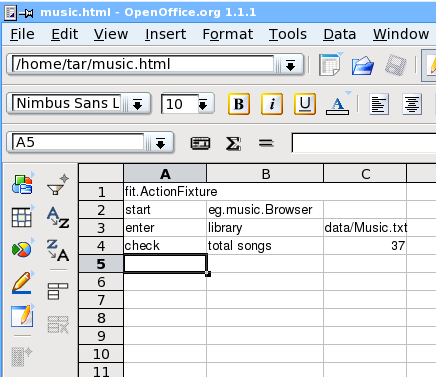
\includegraphics[width=0.35\linewidth]{qm/xfig/testcase-table}
\hfill
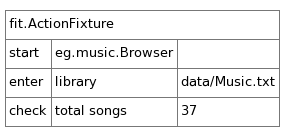
\includegraphics[width=0.45\linewidth]{qm/xfig/testcase-table-html}
%Leider speichert
%der Wordprocessor von OpenOffice (bis und mit Version 2.2)
%die Kopfzeilen von Tabellen (richtigerweise) in th-Elementen ab,
%womit Fit seltsamerweise nichts anfangen kann. Mit MS-Word/Excel
%(oder einer Nach-Editierung) resp. dem Spreadsheet von OpenOffice funktionierts.
\newslide
\item Nun müssen zu jeder Tabelle entsprechende
Fixtures (Spannvorrichtungen) implementiert werden. Das sind Klassen, die
zur Tabelle passende Methoden anbieten und dabei den zu testenden Programmcode
aufrufen.
\begin{lstlisting}[language=java]
public class Browser extends fit.Fixture {
    public void library (String path) throws Exception {
        MusicLibrary.load(path);
    }

    public int totalSongs() {
        return MusicLibrary.library.length;
    }
}
\end{lstlisting}
\newslide
\item Anschliessend können die Tests mit einem einfachen
Kommandozeilenaufruf:
\begin{verbatim}
% java fit.FileRunner input.html output.html
37 right, 10 wrong, 0 ignored, 2 exceptions
\end{verbatim}
ausgeführt werden. Dabei wird die Datei input.html gelesen, die
entsprechenden Tests durchgeführt,
die Test-Ergebnisse in HTML-Format
in die Ausgabedatei
geschrieben und auf der Konsole die Zusammenfassung ausgegeben.
\end{enumerate}

\begin{center}
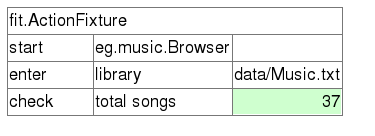
\includegraphics[width=0.45\linewidth]{qm/xfig/testcase-result-html1}
\end{center}
\newslide
Mit Ant kann dafür auch ein Build-Target verwendet werden:
\begin{lstlisting}[language=xml,morekeywords={target,java,arg,classpath}]

   <target name="run"  description="Run Fit">
    <java classname="fit.FileRunner" fork="yes">
          <arg value="input.html"/>
          <arg value="output.html"/>
          <classpath refid="compile.classpath"/>
          <classpath>
              <pathelement path="${build.dir}"/>
          </classpath>
      </java>
   </target>

\end{lstlisting}
%$
\newslide
\begin{figure}[H]
  \centering
\ifslides
  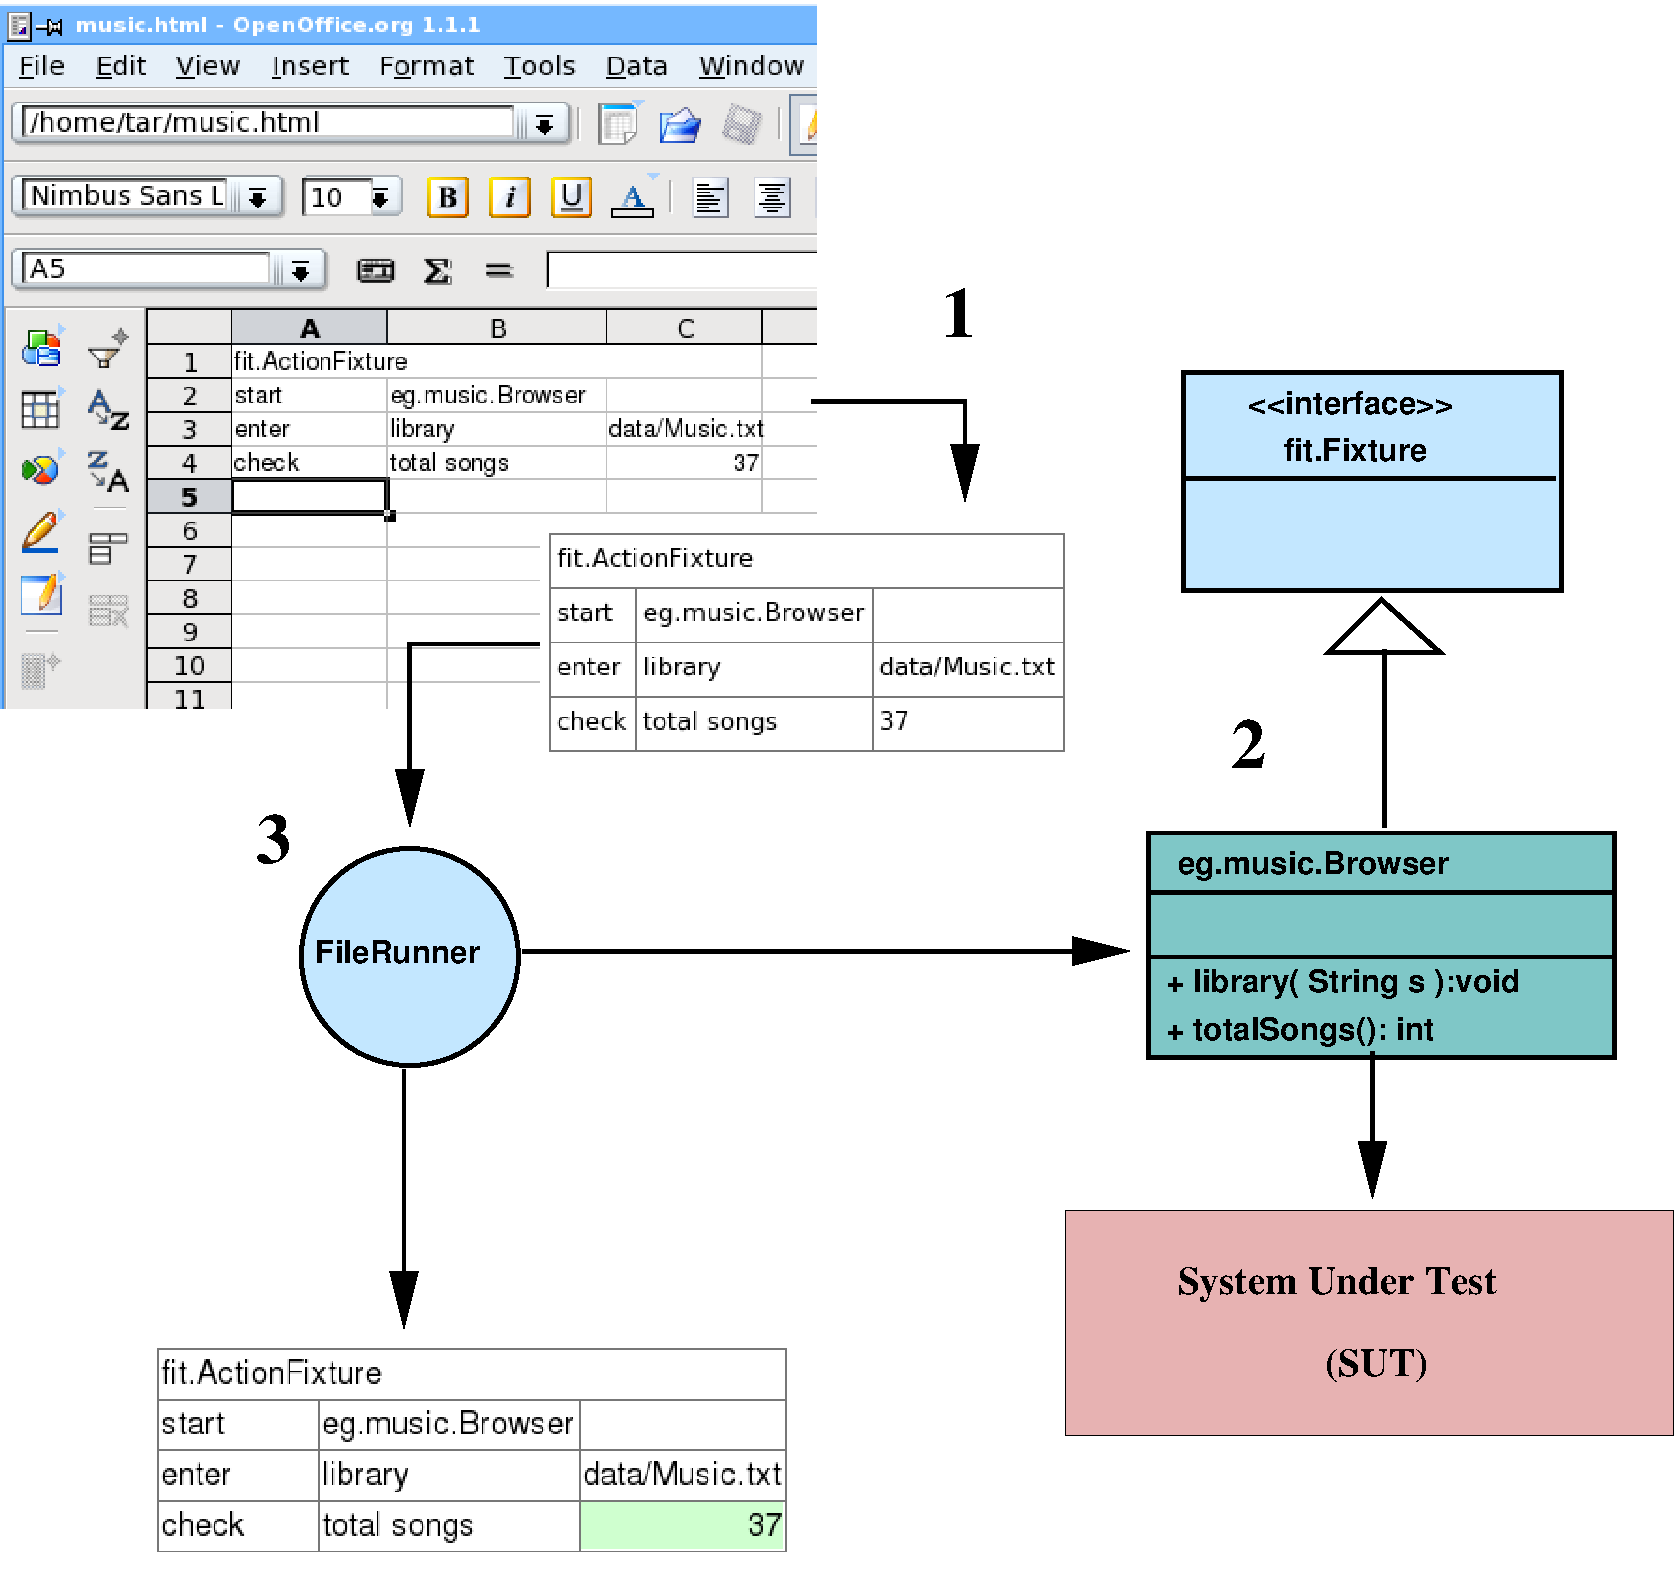
\includegraphics[width=0.7\linewidth]{qm/xfig/fit}
\else
  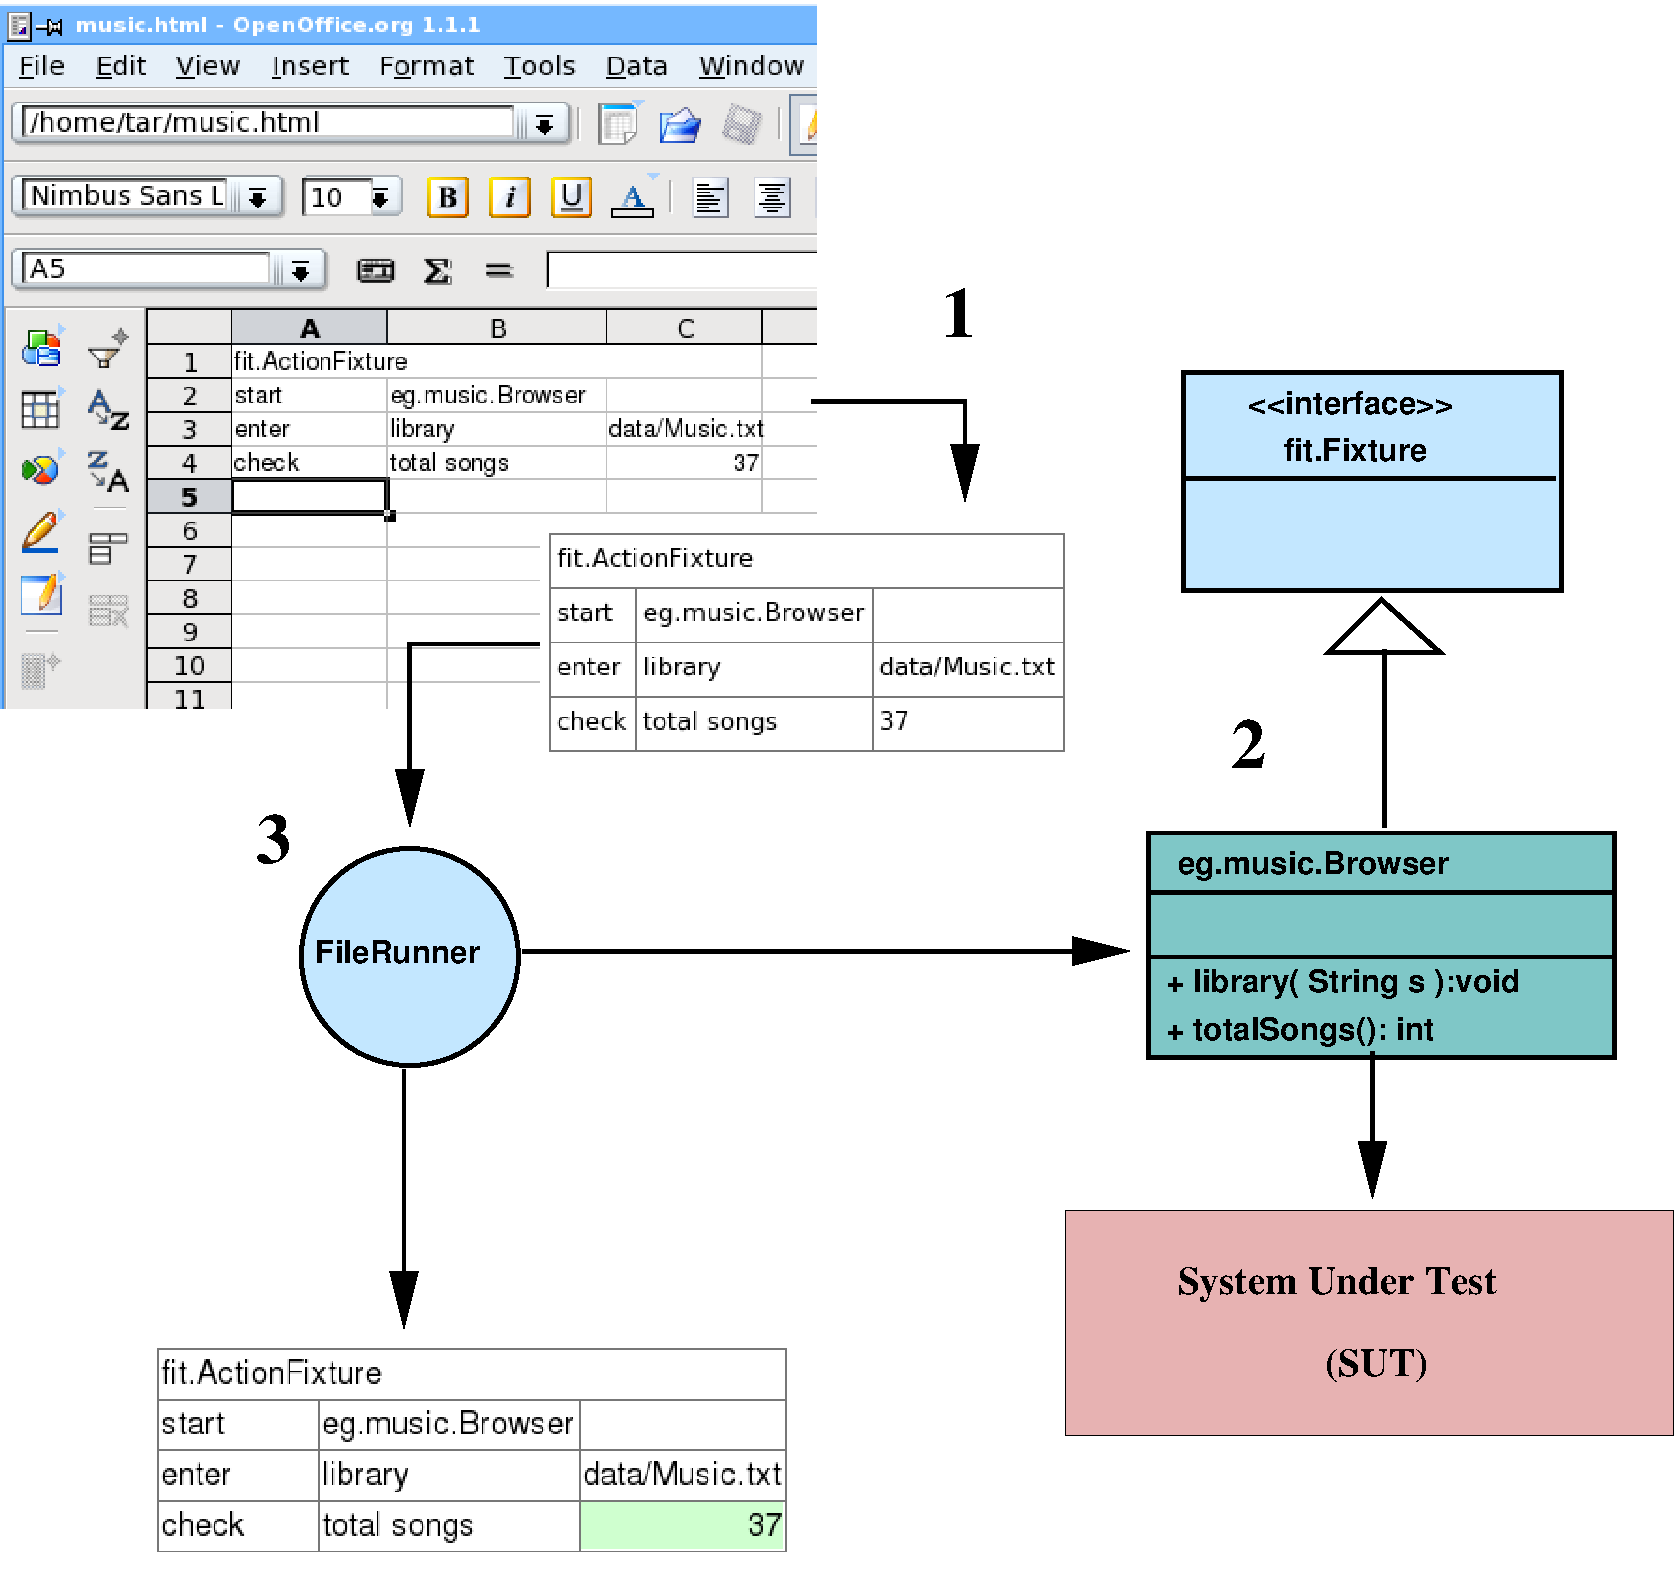
\includegraphics[width=\linewidth]{qm/xfig/fit}
\fi
  \caption{Test-Ablauf mit Fit}
  \label{fig:fit-test-procedure}
\end{figure}
\newslide
Fit unterscheidet unterschiedliche Typen von Fixtures und damit
korrespondierenden Tabellen:
\begin{itemize}
\item \structure{ColumnFixture}: Überprüfung von Regeln und Berechnungen

Die Tabelle besteht aus einer Titelzeile mit dem Klassennamen der Fixture,
einer Kopfzeile mit den Namen der Testdatenparameter und den Zeilen mit den
Testdaten. Ausgaben werden von Eingaben dadurch unterschieden, dass dem
Parameternamen ein Klammerpaar \verb+()+ angehängt wird:
\begin{center}
\begin{tabular}{|l|l|l|}
\hline
\multicolumn{3}{|l|}{\em class name}\\
\hline
{\em param name 1} & {\em param name 2}& {\em \ldots} \\
\hline
{\em value} & {\em value}& {\em \ldots} \\
\ldots & \ldots & \ldots \\
\hline
\end{tabular}
\end{center}
Die Fixture-Klasse muss von fit.ColumnFixture abgeleitet sein, für alle
Eingabeparameter ein gleichbenanntes öffentliches Attribut und für
die Ausgaben eine entsprechende öffentliche Methode enthalten.
%
\newslide
\item \structure{RowFixture}: Überprüfung von Datensätzen

Die Tabelle besteht aus einer Titelzeile mit dem Klassennamen der Fixture,
einer Kopfzeile mit den
Attributbezeichnern des Datensatzes und mehreren Zeilen mit Werten,
wobei die erste Spalte die jeweiligen Schlüsselwerte enthält:
\begin{center}
\begin{tabular}{|l|l|l|}
\hline
\multicolumn{3}{|l|}{\em class name}\\
\hline
{\em key name} & {\em attr name 1}& {\em \ldots} \\
\hline
{\em key value} & {\em value}& {\em \ldots} \\
\ldots & \ldots & \ldots \\
\hline
\end{tabular}
\end{center}
Die Fixture-Klasse muss von RowFixture abgeleitet sein und
die Methoden query und getTargetClass implementiert haben.
Die query-Methode soll die Ergebnisliste zurückgeben und getTargetClass die
Klasse der Ergebnisobjekte. Diese Klasse muss alle in der Tabelle
aufgelisteten Atttribute öffentlich anbieten.
%
\newslide
\item \structure{ActionFixture}: Ausführung einer Sequenz von Anweisungen

Die Tabelle besteht aus einer Titelzeile mit dem Klassennamen
fit.ActionFixture und Zeilen mit zwei resp. drei Spalten:
\begin{center}
\begin{tabular}{|l|l|l|}
\hline
\multicolumn{3}{|l|}{\textbf fit.ActionFixture}\\
\hline
{\em action} & {\em method}& {\em value} \\
\ldots &  & \\
\hline
\end{tabular}
\end{center}
Es stehen die folgenden Aktionen zur Verfügung:
\begin{itemize}
\item start: Erzeugung des Test-Objektes
\item enter: Aufruf von set-Methoden
\item check: Aufruf von get-Methoden und Vergleich mit Sollwert.
\item press: Aufruf von void-Methoden
\end{itemize}
\end{itemize}
Nebst diesen in der Fit-Library enthaltenen können auch eigene Fixture-Klassen
geschrieben werden.
%
\newslide
%\subsection{Integrationstests mit Maven}

Mit Hilfe des Plugins fit-maven-plugin können in der Phase
integration-test Akzeptanztests auf der Basis von Fit durchgeführt werden.
\begin{lstlisting}[language=xml,
morekeywords={plugin,groupId,artifactId,configuration,sourceDirectory,outputDirectory}]
<plugin>
  <groupId>com.googlecode.refit.maven</groupId>
  <artifactId>refit-maven-plugin</artifactId>
  <version>1.7.1</version>

  <configuration>
    <sourceDirectory>src/test/resources</sourceDirectory>
    <outputDirectory>target/fit</outputDirectory>
  </configuration>
</plugin>
\end{lstlisting}
Mit der obigen Konfiguration werden alle im Verzeichnis src/test/fit
abgelegten HTML-Dateien als Eingabe-Argument
 dem Programm fit.FileRunner übergeben. Die Ergebnisdateien werden
 anschliessend ins Verzeichnis target/fit geschrieben.
\newslide
\subsection{FitNesse}
FitNesse ist ein auf Fit basierendes WIKI-System zur Spezifikation von
Anforderungen und Testfällen.
\begin{figure}[H]
\begin{center}
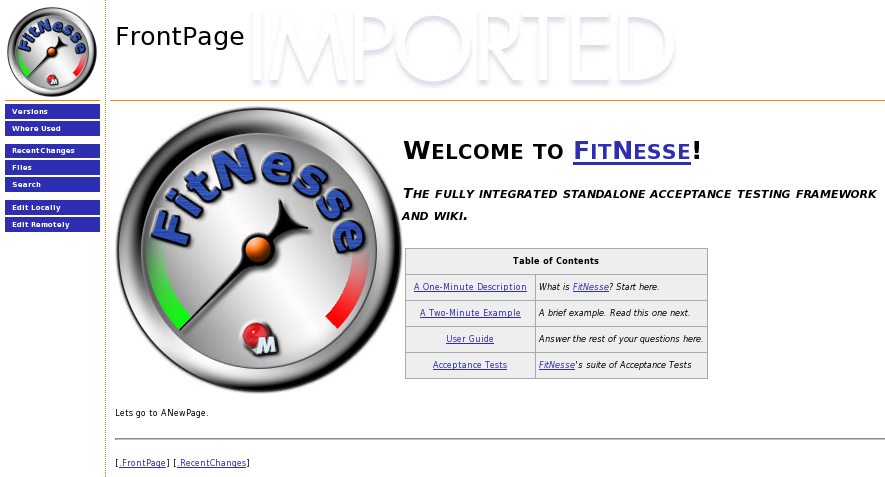
\includegraphics[width=0.8\linewidth]{qm/fitnesse-frontpage}
\caption{Titelseite von FitNesse}
\end{center}
\end{figure}
\newslide
Nach einer kurzen Einführung sind Benutzer in der Lage mit diesem System
Web-Seiten zu erstellen,
die ausführbare Testfälle enthalten:
\begin{figure}[H]
\begin{center}
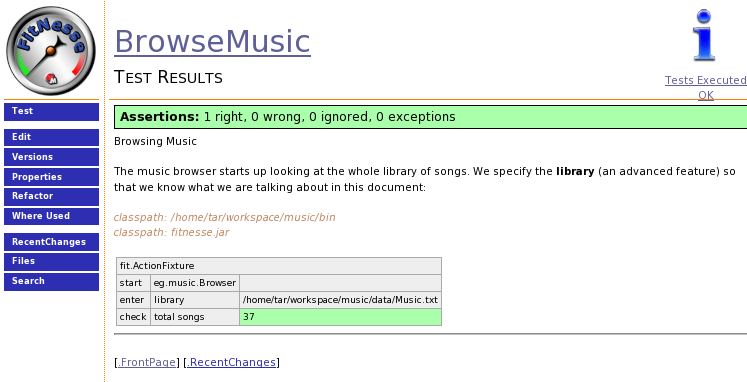
\includegraphics[width=0.8\linewidth]{qm/fitnesse-browsemusic}
\caption{Eine Testseite von FitNesse}
\end{center}
\end{figure}
\newslide
Dazu muss man sich nur ein paar
 wenige Formatierungsanweisungen merken. Zum Beispiel die Definition von
 Tabellen, die den Konzepten von Fit folgen:
\begin{verbatim}
!|fit.ActionFixture|
|start| eg.music.Browser|
|enter| library |/home/tar/workspace/music/data/Music.txt|
|check| total songs |37|
\end{verbatim}
Mittels vertikalen Strichen werden die Spalten und mit path der Klassenpfad
festgelegt:
\begin{verbatim}
!path /home/tar/workspace/music/bin
!path fitnesse.jar
\end{verbatim}
Schliesslich muss mit Properties noch die Eigenschaft Test dieser Seite
hinzugefügt und der Test kann ausgeführt werden, sofern die benötigten
Fixture-Klassen implementiert sind.
%
\newslide
\subsection{JBehave}
JBehave wurde von Dan North entwickelt, weil er zeigen wollte, wie man
Testspezifikationen lesbarer und übersichtlicher machen kann.

Vorgehen:
\begin{enumerate}
\item Man beschreibt in Textdateien die Testfälle in der
BDD-typischen Gherkin-Syntax
  (Beispiel: \lstinline{music_library_scenarios.story})
\begin{lstlisting}[morekeywords={Given, When, And, Then}]
Scenario:  Basic functionality of a Music Library

Given the music library data/Music.txt
When the total of songs is queried
Then the resulting element should be 37
\end{lstlisting}
\newslide
\item Man erstellt die passenden Step-Klassen:
  \begin{lstlisting}[language=java]
public class MusicLibrarySteps {
    int totalSongs;

    @Given("the music library $file")
    public void openLibrary( String file ) {
      ...
    }
    @When("the total of songs is queried")
    public void queryTotalSongs() {
      totalSongs=37;
    }
    @Then("the resulting element should be $result")
    public void theResultingElementShouldBe(int result) {
    	assertThat(totalSongs, equalTo(result));
    }
}
  \end{lstlisting}
\item Man erstellt die JUnitStory-Klasse passend zur Story-Datei
  \begin{lstlisting}[language=java]
public class MusicLibraryScenarios extends JUnitStory {
  @Override
  public Configuration configuration() {
    return new MostUsefulConfiguration()
    // where to find the stories
    .useStoryLoader(new LoadFromClasspath(this.getClass()))
    // CONSOLE and TXT reporting
    .useStoryReporterBuilder(new StoryReporterBuilder()
    .withDefaultFormats()
    .withFormats(Format.CONSOLE, Format.TXT));
  }

  // Here we specify the steps classes
  @Override
  public List<CandidateSteps> candidateSteps() {
    // varargs, can have more that one steps classes
    return new InstanceStepsFactory(configuration(),
                new MusicLibrarySteps()).createCandidateSteps();
  }
  \end{lstlisting}
\item Man führt die Tests mit dem Junit-Testrunner aus.
\end{enumerate}
\newslide
\subsection{Concordion}
Einen ähnlichen Ansatz wie Fit verfolgt Concordion. Die Testfälle
werden in HTML-Format abgelegt und anschliessend von den
Entwicklern mit speziellen Ausführungsanweisungen und
passenden Fixture-Klassen ergänzt. Zur Testausführung wird
JUnit verwendet und die Ergebnisse werden als HTML-Dokument abgespeichert.

\begin{centering}
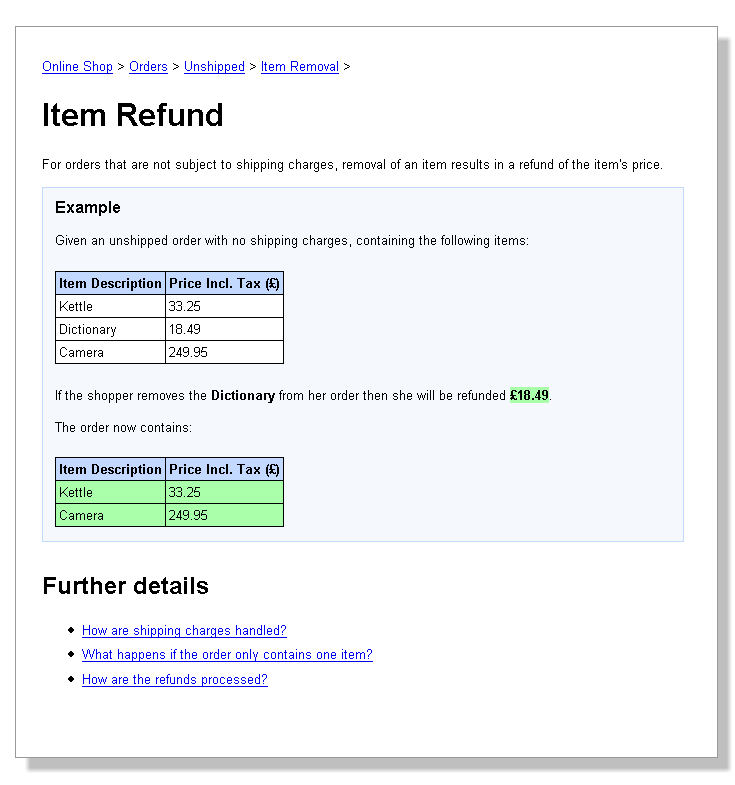
\includegraphics[width=0.8\linewidth]{qm/concordion-itemRefund}
\end{centering}
%

\section{Aufgaben}
\begin{enumerate}
\item Erg"anzen Sie das \verb|LED WebApp| Projekt mit einem Logger.
\item Implementieren Sie an einer geeigneten Stelle im \verb|LED WebApp| Projekt
eine Assertion.
\item Schreiben Sie einen Junit Test f"ur die Methoden \verb|convertTimeStamp| und
\verb|getTimeStamp| der Klasse \verb|TSUtil|.
\item Verwenden Sie eine geeignete Software um zu pr"ufen, zu wie viel Prozent Ihr
Code mit Tests abgedeckt ist.
\item Schreiben Sie zum \verb|LED WebApp| Projekt einen einfachen Test, um die Web Applikation
automatisch zu pr"ufen.
\item Implementieren Sie eine M"oglichkeit, den GPIO Teil von Rasperry PI mit eine MOCK Klasse.
\end{enumerate}

\newslide
\section{Software und weitere Informationen}
\begin{itemize}
\item Software Testing Portal:
\href{http://en.wikipedia.org/wiki/Portal:Software_Testing}
{en.wikipedia.org/wiki/Portal:Software\_Testing}
\item Checkstyle: \href{http://checkstyle.sourceforge.net/}
                         {checkstyle.sourceforge.net/}
\item Log4J: \href{http://logging.apache.org}{logging.apache.org}
\item JUnit \href{http://junit.org}{junit.org}
\item TestNG \href{http://testng.org}{testng.org}
\item EasyMock \href{http://www.easymock.org}{www.easymock.org}
\item Mockito \href{http://mockito.org}{mockito.org}
\item Using Mock Objects in Java (Keld H. Hansen):

  \href{http://javaboutique.internet.com/tutorials/mock_objects}
  {javaboutique.internet.com/tutorials/mock\_objects}
\item Unit Testing with Mock Objects (Ben Teese)

\href{http://www.shinetech.com/display/www/Unit+Testing+with+Mock+Objects}
   {www.shinetech.com/display/www/Unit+Testing+with+Mock+Objects}

\item Designing Testability with Mock Objects (Mario Aquino)

\href{http://www.ociweb.com/jnb/jnbJun2003.html}
  {www.ociweb.com/jnb/jnbJun2003.html}

\item jMock: a library for testing Java code using mock objects

\href{http://jmock.org/index.html}{jmock.org/index.html}

%\item Ant: \href{http://ant.apache.org}{ant.apache.org}
\item Cobertura (Java test coverage)
 \href{http://cobertura.sourceforge.net}
         {cobertura.sourceforge.net}
\item EMMA (Java test coverage)
  \href{http://emma.sourceforge.net}{emma.sourceforge.net}
\item Abbot (framework for automated testing of Java GUI
  components and programs):
  \href{http://abbot.sourceforge.net}{abbot.sourceforge.net}
\item FEST-Swing \href{http://fest.easytesting.org/}
{fest.easytesting.org/}
%\item Jacareto (Java GUI Test ):
%     \href{http://jacareto.sourceforge.net}{jacareto.sourceforge.net}
\item Marathon (Java GUI Test Framework):
   \href{http://marathonman.sourceforge.net}{marathonman.sourceforge.net}
\item JAMon (Performance Tuning and Scalability Measuring):
  \href{http://www.jamonapi.com}{www.jamonapi.com}
\item JUnitPerf (Performance and Scalability testing with JUnit)
  \href{http://clarkware.com/software/JUnitPerf.html}{clarkware.com/software/JUnitPerf.html}
%\item EJP (Extensible Java Profiler):
%  \href{http://ejp.sourceforge.net}{ejp.sourceforge.net}
\item Test and Performance Tools Platform:
  \href{http://www.eclipse.org/tptp}{www.eclipse.org/tptp}
\item The Grinder (Java Load Testing Framework):
   \href{http://grinder.sourceforge.net}{grinder.sourceforge.net}
\item Valgrind: (Speichertests)
    \href{http://valgrind.org/}{valgrind.org/}
\item C/C++ Unittesting
  HOWTO:
\href{http://www.sipfoundry.org/developer-tools/c/c-unittesting-howto.html}
              {www.sipfoundry.org/developer-tools/c/c-unittesting-howto.html}
\item DseWiki: Speicher Checker:
  \href{http://www.wikiservice.at/dse/wiki.cgi?SpeicherChecker}
    {www.wikiservice.at/dse/wiki.cgi?SpeicherChecker}
\item JMeter
  \href{http://jakarta.apache.org/jmeter}{jakarta.apache.org/jmeter}
\item Stress testing an application with JMeter (Daniel Rubio, Feb 2004)\\
  \href{http://www.newsforge.com/software/04/02/19/1452218.shtml}
            {www.newsforge.com/software/04/02/19/1452218.shtml}
\item JMeter-Ant-Task: \href{http://www.programmerplanet.org/ant-jmeter/}
     {www.programmerplanet.org/ant-jmeter/}
%%\item CruiseControl: Automatisiertes Testen und Erstellen:
\href{http://cruisecontrol.sourceforge.net}{cruisecontrol.sourceforge.net}

\item Hudson: Extensible continuous integration server:
\href{http://jenkins-ci.org}{jenkins-ci.org}
%
\item Java Extreme Programming Cookbook (Eric M. Burke, Brian M. Coyner):

  \href{http://www.oreilly.com/catalog/jextprockbk}
      {www.oreilly.com/catalog/jextprockbk}
%
\item Findbugs:
  \href{http://findbugs.sourceforge.net}{findbugs.sourceforge.net}
\item PMD:
  \href{http://pmd.sourceforge.net/}{pmd.sourceforge.net/}
\item Fit: \href{http://fit.c2.com}{fit.c2.com}
\item FitNesse: \href{http://fitnesse.org}{fitnesse.org}
\item Programming Tools: FitNesse (Reg. Charney)

\href{http://www.linuxjournal.com/article/8482}
    {www.linuxjournal.com/article/8482}
\item Wiki-getriebene Akzeptanztests (Josef Adersberger):

\href{http://javamagazin.de/itr/online_artikel/psecom,id,787,nodeid,11.html}
     {javamagazin.de/itr/online\_artikel/psecom,id,787,nodeid,11.html}

%\item Ein Eclipse-Plugin für Fit:
%
%\href{http://fitrunner.sourceforge.net}{fitrunner.sourceforge.net}

\item Web-Testing mit Selenium:

\href{http://www.openqa.org/selenium}{www.openqa.org/selenium}
%
\item Web-Testing mit Canoo:

\href{http://webtest.canoo.com/webtest/manual/WebTestHome.html}
{webtest.canoo.com/webtest/manual/WebTestHome.html}

\item Data-Driven Tests:
  \href{http://www.ddsteps.org}{www.ddsteps.org}
\item EasyB \href{http://www.easyb.org}{www.easyb.org}
\item Concordion \href{http://www.concordion.org}{www.concordion.org}
\item JBehave \href{http://jbehave.org/}{jbehave.org/}
\item RobotFramework \href{http://code.google.com/p/robotframework}{code.google.com/p/robotframework}
\end{itemize}
% code checking tools:
% http://www.tiobe.com/
%
% http://jcsc.sourceforge.net/
% JTest http://www.parasoft.com/jsp/products/home.jsp?product=Jtest&itemId=11
% JStyle ?
%
% http://en.wikipedia.org/wiki/GUI_testing
%
%%% Local Variables:
%%% mode: latex
%%% TeX-master: "cvs-aufgaben"
%%% End:
